\documentclass{article}
\usepackage{cite}
\usepackage{color}
\usepackage{float}
\usepackage{caption}
\usepackage{amsmath}
\usepackage{graphicx}
\usepackage{listings}
\usepackage{subcaption}
\usepackage[T1]{fontenc}
\usepackage[polish]{babel}
\usepackage[utf8]{inputenc}

\definecolor{dkgreen}{rgb}{0,0.6,0}
\definecolor{gray}{rgb}{0.5,0.5,0.5}
\definecolor{mauve}{rgb}{0.58,0,0.82}

\lstset{frame=tb,
  language=Python,
  aboveskip=3mm,
  belowskip=3mm,
  showstringspaces=false,
  columns=flexible,
  basicstyle={\small\ttfamily},
  numbers=none,
  numberstyle=\tiny\color{gray},
  keywordstyle=\color{blue},
  commentstyle=\color{dkgreen},
  stringstyle=\color{mauve},
  breaklines=true,
  breakatwhitespace=true,
  tabsize=4
}

\title{Segmentacja komórek na zdjęciach mikroskopowych skóry z użyciem głębokich sieci neuronowych.}
\date{2020-12-25}
\author{Michał Tracewicz}
\begin{document}
\maketitle
\newpage
\tableofcontents
\newpage
\section{Wstęp}
W codziennej pracy wielu lekarzy poświęca czas na manualne liczenie zafarbowanych komórek na zdjęciach.
Jest to czasochłonne i monotonne zadanie.
Zdecydowanie nie należy ono do takich, które wymagają sześcioletnich studiów.
Co za tym idzie, nadaje się ono idealnie do automatyzacji.

W ostatnich latach bardzo mocno rozwija się dziedzina uczenia maszynowego.
Technika ta jest inspirowana działaniem ludzkiego mózgu i pozwala na pisanie programów dla, których trudno jest zdefiniować jednoznaczny zbiór reguł postępowania.
Człowiek posiada pewną intuicję dzięki, której jest w stanie w dość krótkim czasie nauczyć się w jaki sposób należy obrysować komórkę.
Jednakże gdy zostanie poproszony o wyjaśnienie swojego podejścia będzie to trudne lub wręcz nie wykonalne.
Możemy się raczej spodziewać odpowiedzi pokroju ``No patrzę na komórkę i ją obrysowuje''.
Biorąc pod uwagę specyfikę tego problemu użycie tej metody wydaję się idealne.

W ramach mojej pracy przeprowadziłem testy architektury U-Net będącej jedną z najpopularniejszych wyborów do zadań związanych z segmentacją obrazów medycznych.
Przetestowałem również różne rodzaje obróbki obrazów wyjściowych w celu zwiększenia skuteczności działania sieci.

Dodatkowo stworzyłem również zestaw narzędzi pozwalający na łatwe testowanie różnych architektur oraz funkcji strat dla sieci neuronowych w tym problemie.
Rozwiązanie zostało napisane w języku Python\footnote{https://www.python.org/} z użyciem następujących bibliotek
\begin{itemize}
    \item Keras\footnote{https://keras.io/} - służy do pracy z sieciami neuronowymi i jest interfejsem do biblioteki TensorFlow
    \item TensorFlow\footnote{https://www.tensorflow.org/} - biblioteka ta pozwala na wykonywanie obliczeń na tensorach
    \item NumPy\footnote{https://numpy.org/} - biblioteka do obliczeń numerycznych na n-wymiarowych tablicach
    \item Pillow\footnote{https://python-pillow.org/} - biblioteka pozwalająca na wczytywanie, zapisywanie oraz edycję obrazów.
    \item Jupyter Notebook\footnote{https://jupyter.org/} - pozwalająca utworzyć interaktywne środowisko uruchomieniowe Python-a w przeglądarce.
\end{itemize}
Kod źródłowy projektu jest wersjonowany z użyciem narzędzia git\footnote{https://git-scm.com/} \newline oraz upubliczniony na platformie GitHub\footnote{https://github.com/mtracewicz/CellSegmentation/}.
Prezentacja wyników jest dostępna online za pośrednictwem platformy GitHub Pages\footnote{ https://mtracewicz.ksummarized.com/CellSegmentation.}
Repozytorium zawierające kod projektu zostało podłączone do platformy CircleCi\footnote{https://circleci.com/} w celu automatycznego uruchamiania testów jednostkowych (napisane przy użyciu PyTest\footnote{https://docs.pytest.org/en/latest/} i Tox\footnote{https://tox.readthedocs.io/en/latest/}) oraz publikacji wyników.
W ramach pracy powstały również skrypty w powłoki bash\footnote{https://www.gnu.org/software/bash/} tworzące kontener deweloperski (technologia Docker\footnote{https://www.docker.com/}) zawierający wszystkie niezbędne biblioteki.
Całość dopełnia moduł pozwalający na obróbkę zdjęć wejściowych oraz wyjściowych.

Jako, że obrazy medyczne są danymi chronionymi prawnie to szpitale w większości wypadków nie mogą wysłać ich poza własną sieć wewnętrzną.
Z tego powodu przetestowałem również możliwość uruchomienia splotowej sieci neuronowej w przeglądarce z użyciem biblioteki TensorFlowJS\footnote{https://www.tensorflow.org/js}.
Dzięki takiemu podejściu jedynie uczenie modelu przebiega na komputerze nie będącym komputerem klienckim.
Model zostaje nauczony na jednym komputerze ale predykcja dla konkretnego obrazu wejściowego wykonywana jest w przeglądarce po stronie klienta (nie następuje wysłanie zapytania do serwera API) i nigdy nie opuszcza sieci.
\subsection{Obrazy wejściowe i wyjściowe}
W opracowywanym przeze mnie zagadnieniu jako obrazy wejściowe użyte zostały zdjęcia mikroskopowe skóry.
Wszystkie zdjęcia są zrobione z przybliżeniem x40 oraz posiadają rozmiar 1200x1600px z trzema kanałami.
Obrazy wyjściowe zostały przygotowane za pomocą programu opracowany przez Panią Dominikę Pawłowską.
Są to obrazy tego samego rozmiaru jednak zawierają cztery kanały zamiast trzech (RGBA zamiast RGB).
Możemy na nich zobaczyć czerwoną otoczkę na około komórek, natomiast cała reszta obrazu jest przezroczysta.
\begin{figure}[H]
    \centering
    \begin{subfigure}{0.4\linewidth}
        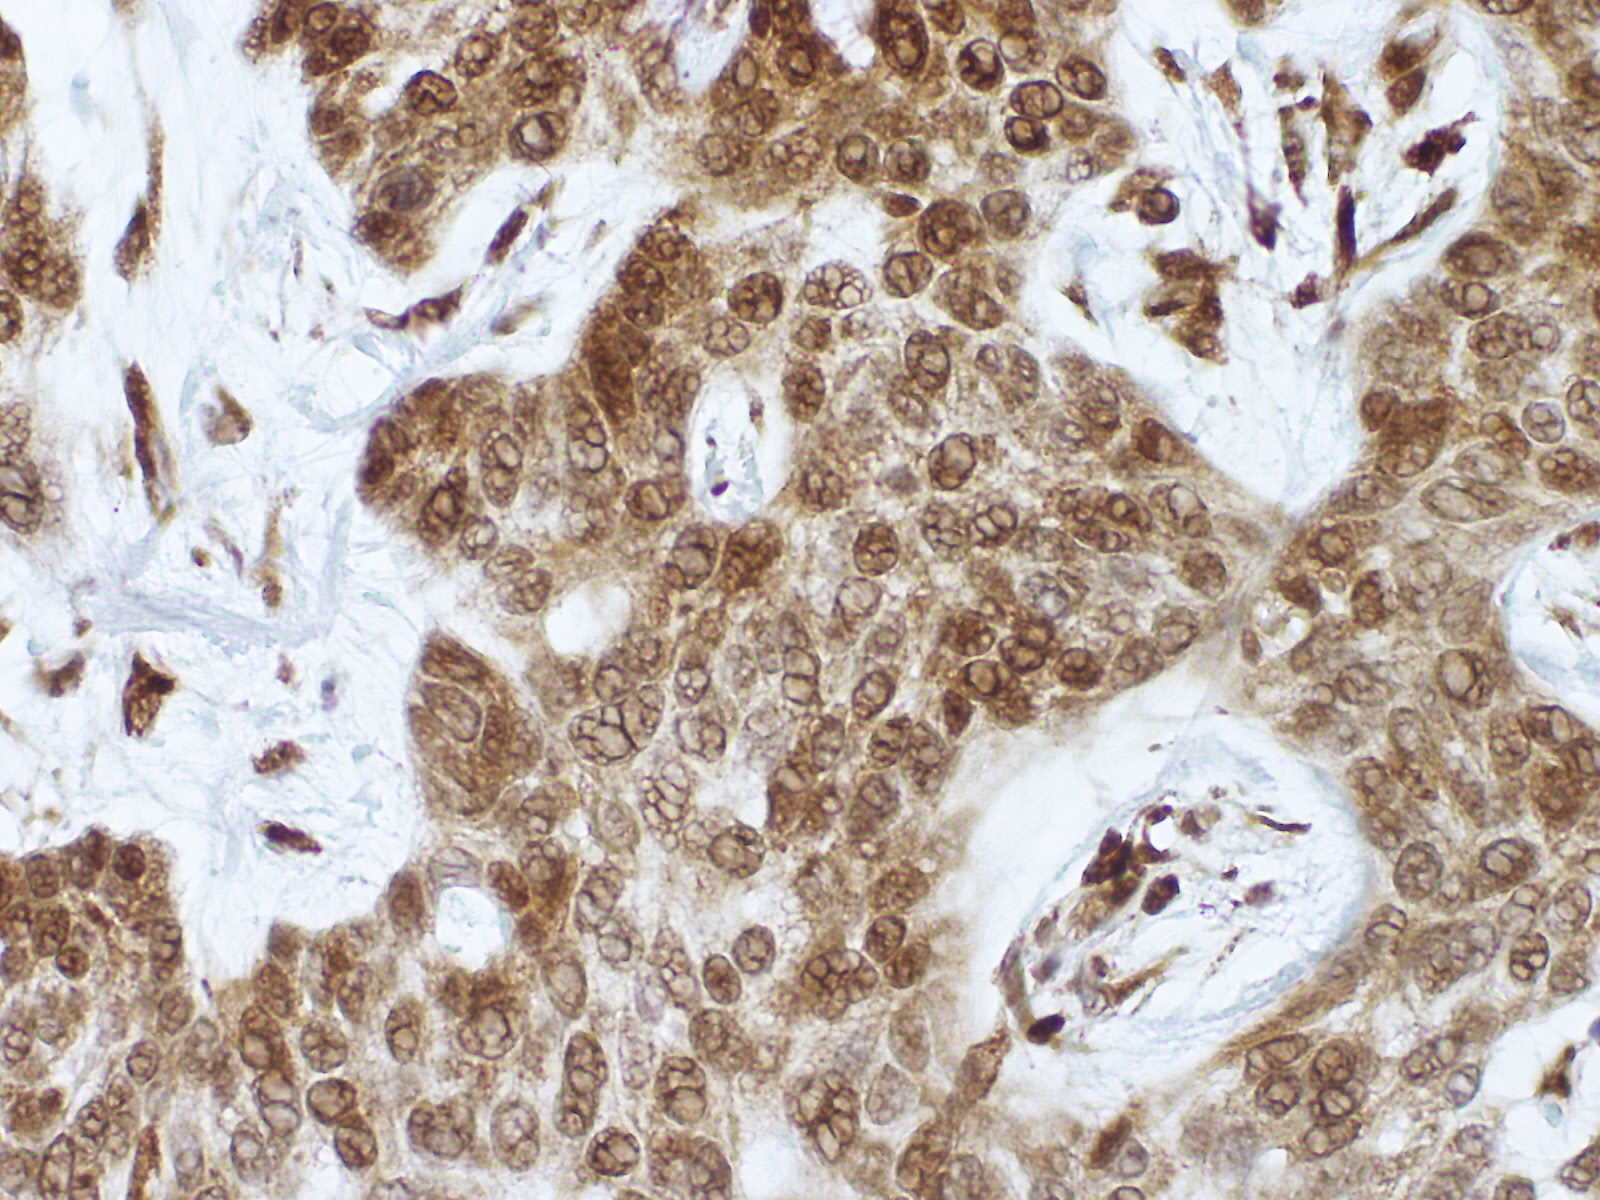
\includegraphics[width=\linewidth]{images/input.png}
        \caption{Wejście}
    \end{subfigure}
    \begin{subfigure}{0.4\linewidth}
        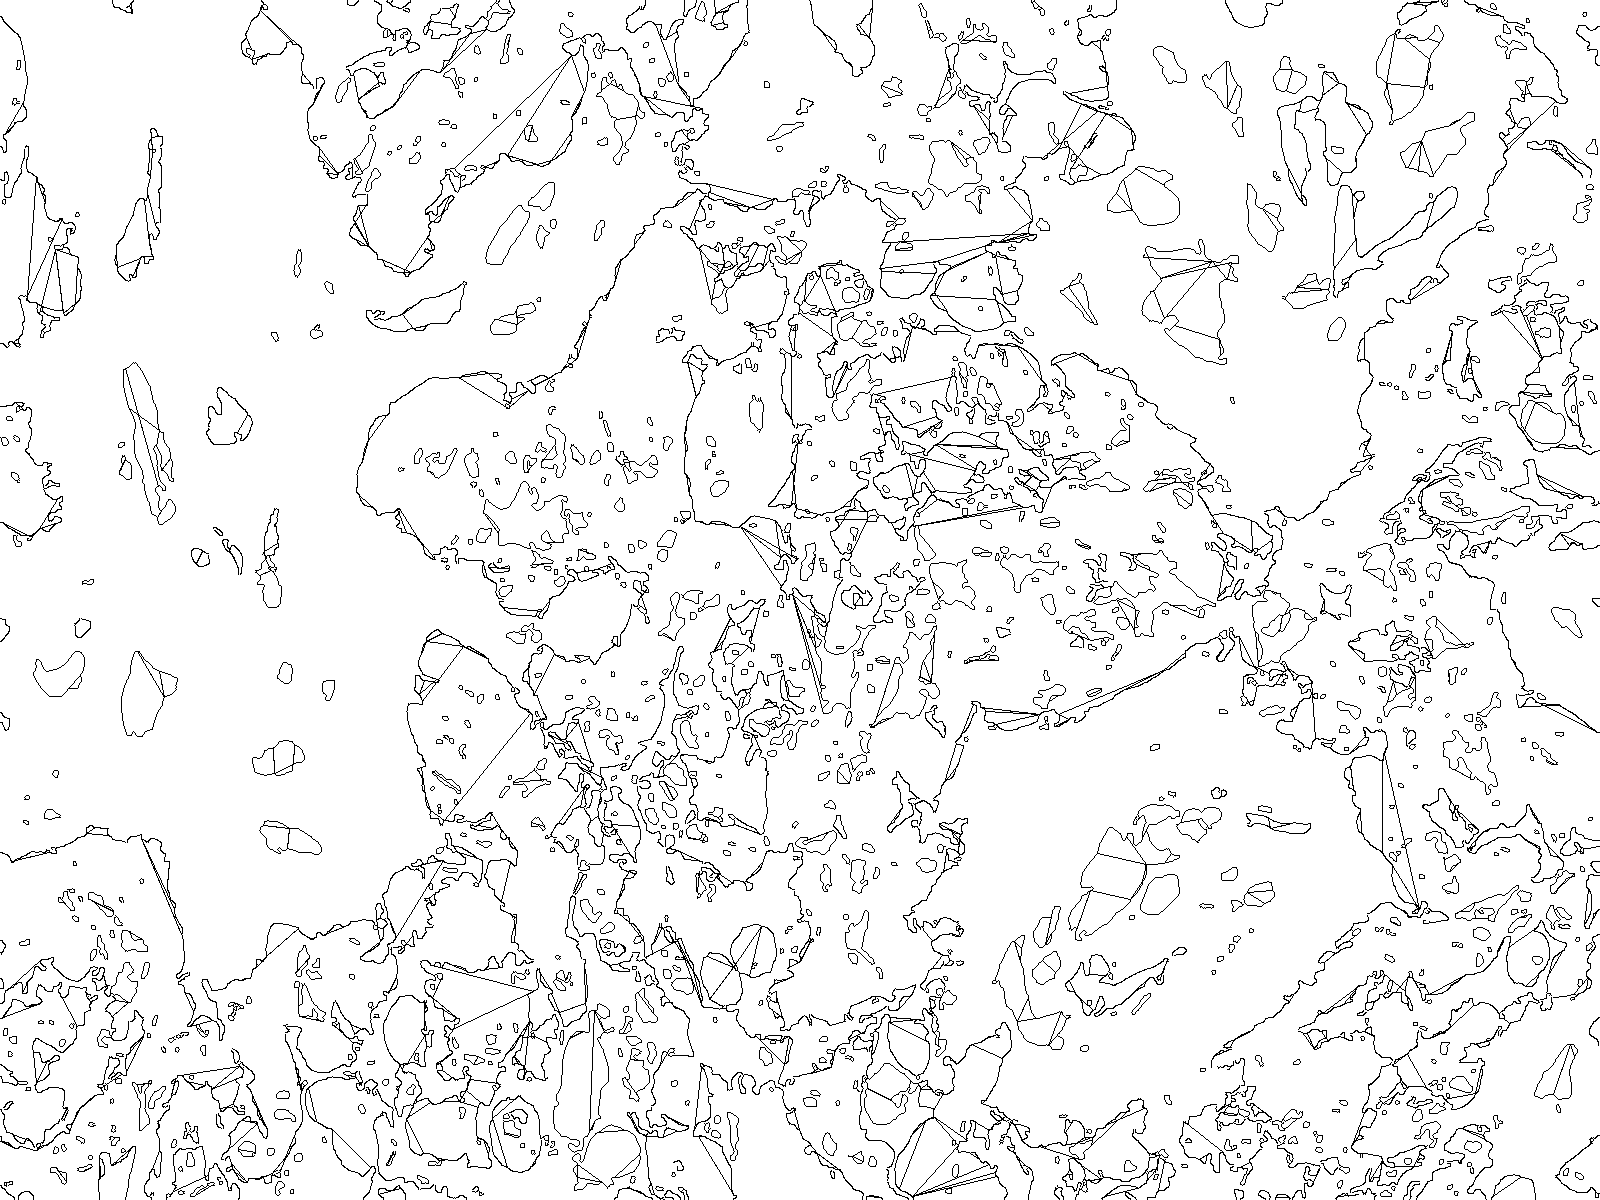
\includegraphics[width=\linewidth]{images/output.jpg}
        \caption{Wyjście}
    \end{subfigure}
    \caption{Przykładowe obrazy wejściowy i wyjściowy}
    \label{fig:input_and_output}
\end{figure}
\newpage
\section{Sztuczne sieci neuronowe}
Sztuczne sieci neuronowe są próbą stworzenia programów, których działanie jest inspirowane naszym rozumieniem mózgu.
Chociaż zagadnienie to podejmowano już od bardzo długiego czasu, to dopiero od niedawna posiadamy wystarczającą moc obliczeniową aby realizować tworzone od wielu dziesięcioleci algorytmy.

\subsection{Ogólne zasady działania}
Głębokie sieci neuronowe składają się z warstwy wejściowej, wyjściowej oraz pewnej liczby warstw ukrytych.
Każda warstwa składa się z neuronów, które przyjmują wartość zależnie od wyniku funkcji aktywacyjnej.
Liczba oraz typ warstw ukrytych a także ilość zawartych w nich neuronów w dużej mierze determinuje działanie sieci.

Omówienie zaczniemy od tego w jaki sposób sieć przeprowadza obliczenia zwracające odpowiedź, a następnie zajmiemy się procesem uczenia.
Neurony kolejnych warstw są ze sobą połączone (zajmę się tu jedynie warstwami, które posiadają połączenia neuronów każdy z każdym, czyli tak zwanymi warstwami typu ``dense``).
Połączenia te posiadają wagi.
Aby obliczyć wynik zwracany przez sieć rozpoczynamy obliczenia od warstwy wejściowej i obliczmy wartości neuronów w kolejnych warstwach.
Wartość dla neuronu w warstwie k-tej to wartość funkcji aktywacji na sumie wartości wszystkich neuronów z warstwy poprzedniej przemnożonych przez odpowiednie im wagi połączeń.
\begin{align*}
    x_{k,j} = \sigma(\sum\limits_{i=0}^{n-1}{w_ix_{(k-1),i}})
\end{align*}
Gdzie (k>=1):
\begin{itemize}
    \item $\sigma$ - funkcja aktywacji
    \item $x_{k,j}$ - wartość j-tego neuronu w k-tej warstwie
    \item n - liczba neuronów w warstwie k-1
    \item $w_i$ - i-ta waga wchodząca do neuronu
\end{itemize}
Obliczając w ten sposób wartości wszystkich neuronów w ostatniej - warstwie wyjściowe otrzymujemy odpowiedź naszego modelu.

Proces uczenia to wielorazowe przejście przez poprawnie opisane dane wejściowe i poprawianie wag w celu minimalizacji funkcji błędu.
W celu poprawy wag używamy algorytmu wstecznej propagacji błędu.
Polega on na poprawianiu wag poprzez przejście sieci w przeciwnym kierunku i zmianie wartości wag na podstawie delt wyliczonych przy pomocy algorytmu spadku gradientowego.

\subsection{Porównanie do klasycznych metod programowania}
Przy standardowych paradygmatach programowania (programowanie zorientowane obiektowo, programowanie proceduralne, programowanie funkcyjne) jako programista piszemy kod, który
instruuje komputer na temat tego w jaki sposób ma on przekształcić otrzymane dane wejściowe.
Natomiast sieci neuronowe są zdecydowanie bardziej zbliżone do programowania deklaratywnego. Jako programista podajemy dane wejściowe, architekturę i oczekiwane dane wyjściowe i na ich podstawie, chcemy aby komputer samemu ``nauczył się`` tego jaką drogą ma dojść aby uzyskać oczekiwany efekt (jakie wartości mają przyjmować wagi).
\newpage
\section{Sieci splotowe}
Sieci splotowe to takie głębokie sieci neuronowe, które zawierają jedną lub więcej warstw splotowych.
\subsection{Operacja splotu}
Operacja splotu w kontekście sieci neuronowych jest to przebieg jądra przez wartości pikseli obrazu wejściowego.
W przestrzeni dwu wymiarowej jest to równoważne z nałożeniem na obraz wejściowy filtra.
\subsection{Sieci w pełni splotowe}
Sieciami w pełni splotowymi nazywamy te głębokie sieci neuronowe, które jako wszystkie warstwy posiadają warstwy splotowe.
Sieci tego typu służą głównie do przekształcania obrazów.
\newpage
\section{Problem segmentacji}
Uczenie maszynowe możemy podzielić na różne podtypy.
Jednym z nich jest zagadnienie wizji komputerowej.
Zaznaczenie konturów komórek na zdjęciach mikroskopowych jest problemem segmentacji instancji, która jest częścią tego zagadnienia.
W celu zrozumienia tego pojęcia przeanalizujemy składające się na niego mniejsze problemy z kategorii widzenia komputerowego.
\subsection{Klasyfikacja}
Jest to najprostsze zagadnienie w dziedzinie widzenia komputerowego.
Polega ono na tym, że dla otrzymanego na wejście obrazu sieć ma zwrócić klasę do której przedstawiony na zdjęciu obiekt należy.
Za dobry przykład może nam posłużyć ``Problem MNiST``, polegający na rozpoznawaniu odręcznie napisanych cyfr.
Jako wejście sieć otrzymuje czarno-biały obrazek rozmiaru 16x16 pikseli na, którym widnieje odręcznie napisana cyfra.
Natomiast na wyjściu sieć zwraca nam predykcję jaka cyfra widnieje na zdjęciu.
Ograniczeniem w tym typie problemu jest fakt, że na danym zdjęciu może znajdować się jedynie pojedyńczy obiekt.
\begin{figure}[H]
    \centering
    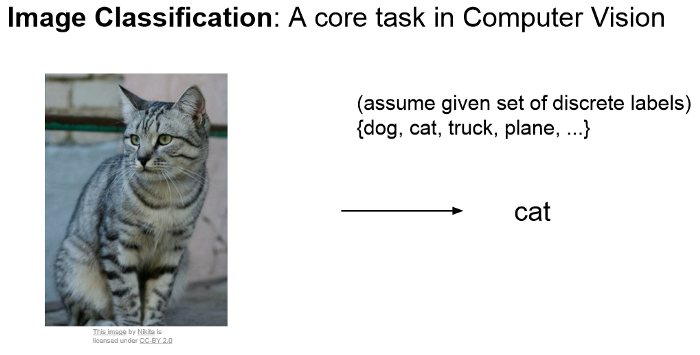
\includegraphics[width=\linewidth]{images/klasyfikacja.png}
    \caption{Przykład klasyfikacji}
    \label{fig:klasyfikacja}
\end{figure}
\subsection{Klasyfikacja z lokalizacją}
Klasyfikacja z lokalizacją to dodanie do poprzedniego problemu zagadnienia odnalezienia klasyfikowanego obrazu na zdjęciu.
Przykładowo tworząc sieć rozpoznającą gatunki zwierząt domowych, otrzymując zdjęcie kota siedzącego na kanapie otrzymamy nie tylko informację,
że jest to kot ale również informację o tym gdzie na tej kanapie się znajduje.
Najczęściej zwracane są w takim wypadku oprócz klasy współrzędne pikseli w których zaczyn i kończy się obiekt.
Następnie możemy na tej podstawie narysowanie naokoło obiektu ramkę z podpisem zawierającym nazwę klasy.
\begin{figure}[H]
    \centering
    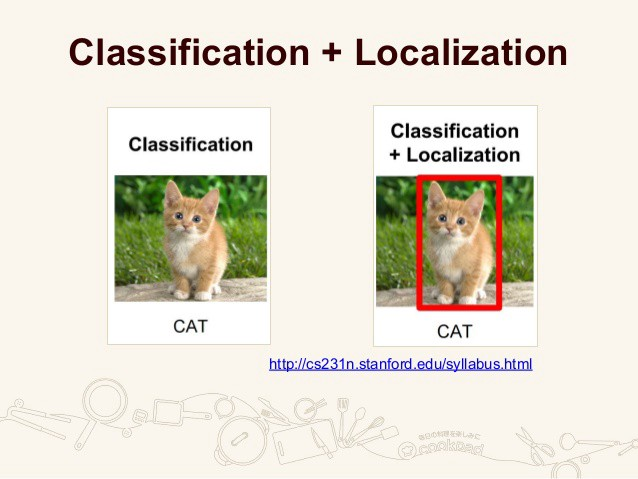
\includegraphics[width=\linewidth]{images/klasyfikacja_z_lokalizacja.jpeg}
    \caption{Przykład klasyfikacji z lokalizacją}
    \label{fig:klasyfikacja_z_lokalizacja}
\end{figure}
\subsection{Wykrywanie obrazów}
Kolejnym krokiem jest wykrywanie obrazów. Jest to klasyfikacja z lokalizacją dla wielu elementów jednocześnie.
Kontynuując poprzedni przykład z rozpoznawaniem zwierząt domowych.
W wypadku zdjęcia, które zawiera zarówno psa i kota dostaniemy zestaw współrzędnych oraz odpowiadających im klas.
\begin{figure}[H]
    \centering
    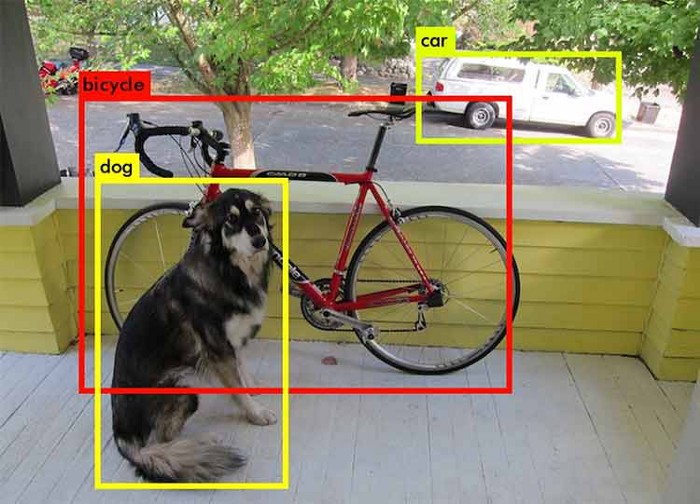
\includegraphics[width=\linewidth]{images/detekcja.jpeg}
    \caption{Przykład wykrywania obrazów}
    \label{fig:wykrywanie_obrazow}
\end{figure}
\subsection{Segmentacja}
Segmentacja to przypisanie każdemu pikselowi na obrazie wejściowym klasy.
Za przykład może nam posłużyć zdjęcie drogi w mieście.
Celem naszej sieci neuronowej będzie podział obrazu na klasy: droga, człowiek, budynek, drzewo, niebo etc.
Na wyjściu możemy na przykład otrzymać ten sam obrazek z tym, że zależnie od klasy danego piksela będzie miał on różny kolor (czerwony - droga, zielony - człowiek etc.)
\begin{figure}[H]
    \centering
    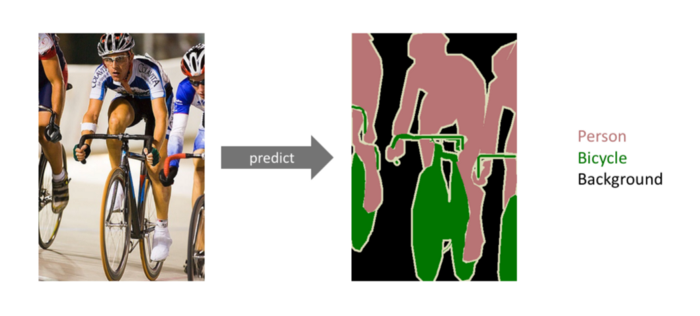
\includegraphics[width=\linewidth]{images/segmentacja.png}
    \caption{Przykład segmentacji}
    \label{fig:segmentacja}
\end{figure}
\subsection{Segmentacja instancji}
Segmentacja instancji to dodanie do segmentacji ograniczenia, że każda jednostka ma być widocznie oddzielona.
Dla przykładu gdy mamy zdjęcie czterech przytulających się osób, w wyniku segmentacji wszystkie cztery zostaną zakolorowane na ten sam kolor oraz podpisane raz jako człowiek.
Natomiast gdy przeprowadzimy segmentację instancji to w wyniku otrzymamy każdą osobę pokolorowaną na własny kolor, oraz etykiety ``człowiek 1.``, ``człowiek 2.`` etc.
\begin{figure}[H]
    \centering
    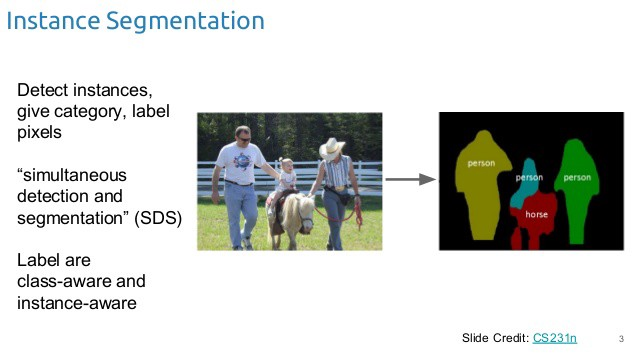
\includegraphics[width=\linewidth]{images/segmentacja_instancji.jpeg}
    \caption{Przykład segmentacji instancji}
    \cite{patashnik-bibtexing}
    \label{fig:segmentacja_instancji}
\end{figure}
\newpage
\section{Architektura U-Net historia i zastosowania}
\newpage
\section{Przetestowane podejścia}
W ramach pracy przetestowałem architekturę U-Net oraz różne podejścia do obróbki danych.
Mimo wielu prób sieci które przygotowałem zawsze zwracały niemal w pełni czarne/czerwone obrazy.
\begin{figure}[H]
    \centering
    \begin{subfigure}{0.4\linewidth}
        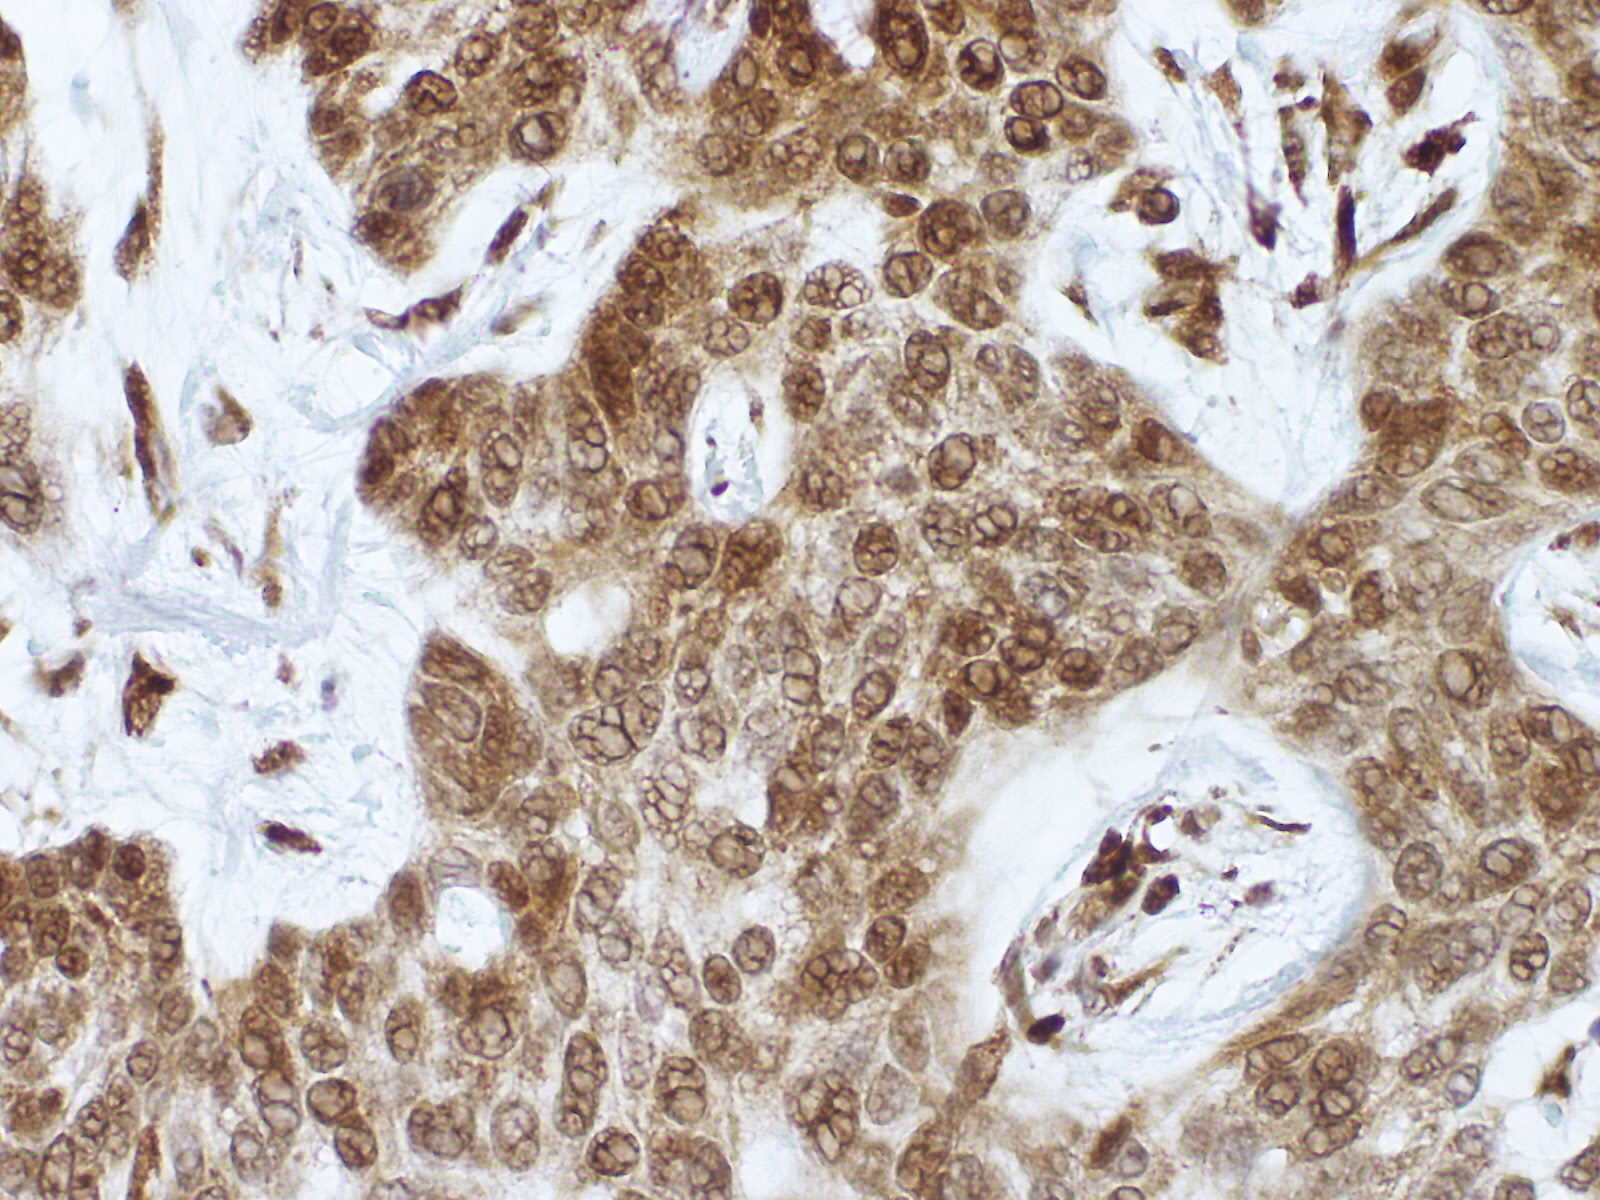
\includegraphics[width=\linewidth]{images/input.png}
    \end{subfigure}
    \begin{subfigure}{0.4\linewidth}
        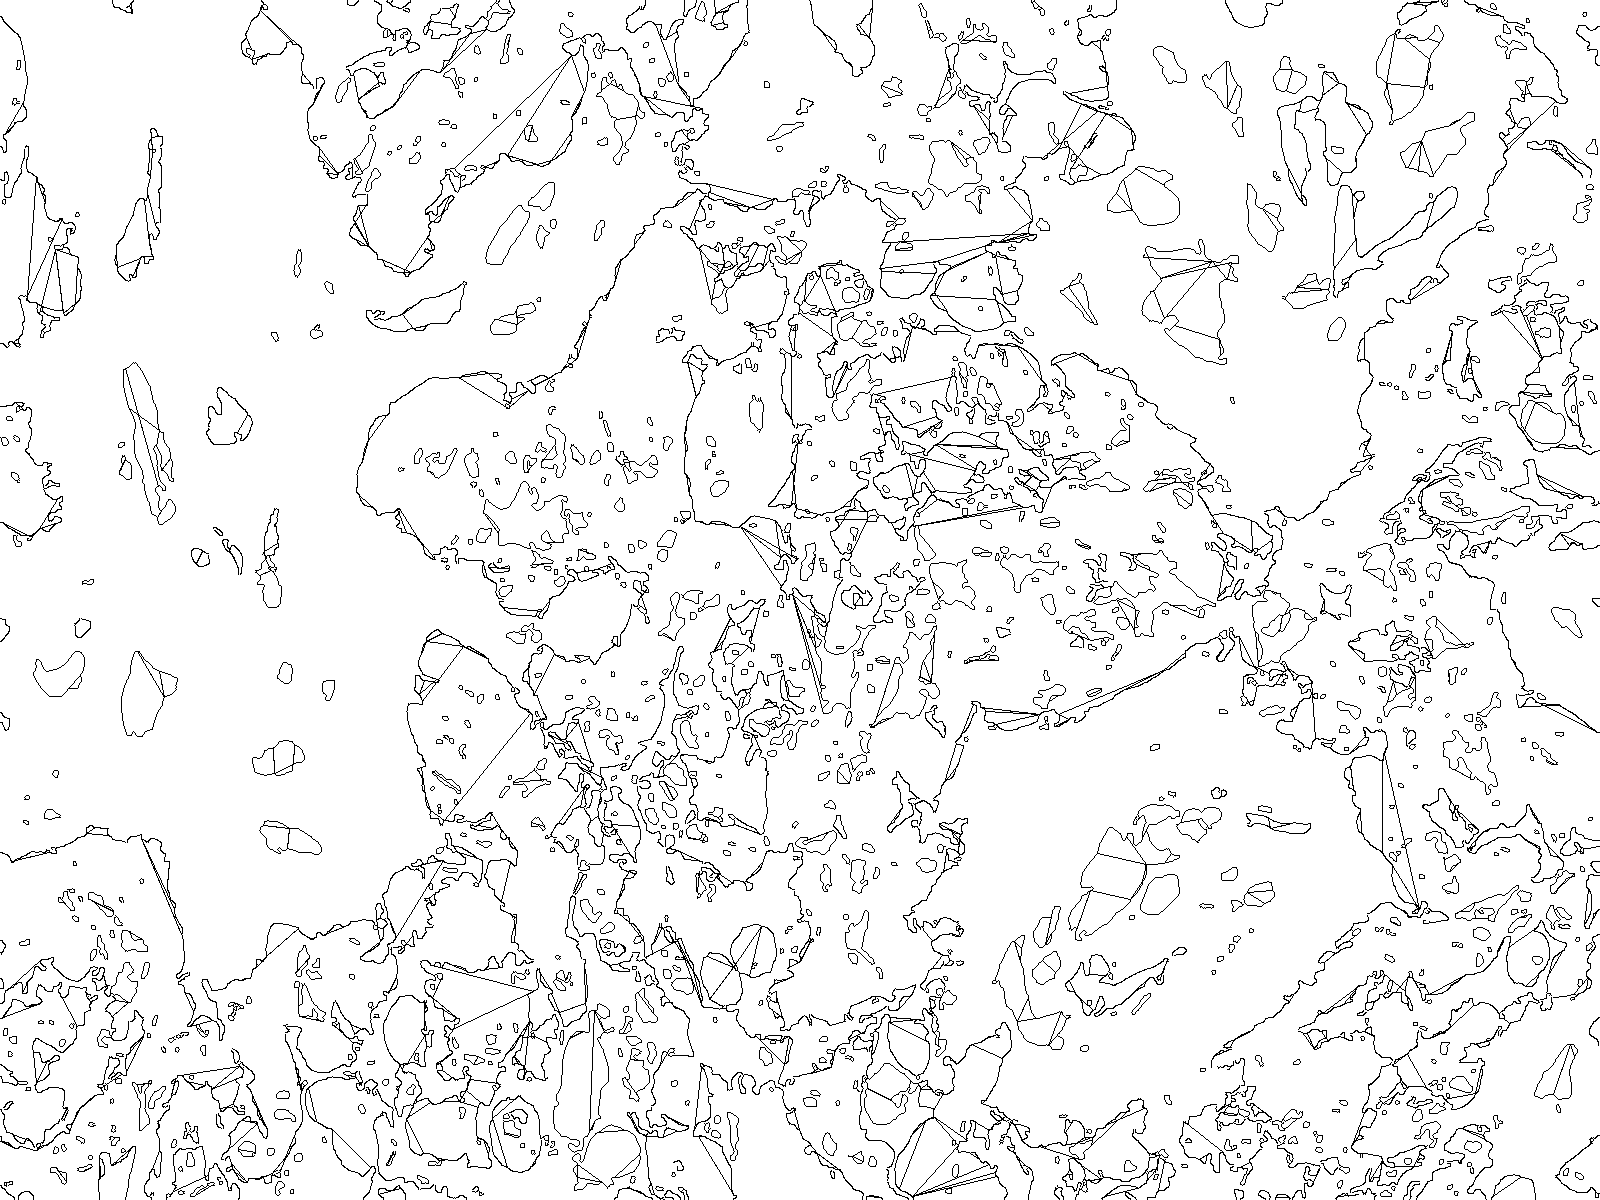
\includegraphics[width=\linewidth]{images/output.jpg}
    \end{subfigure}
    \caption{Przykładowe otrzymane wyniki}
    \label{fig:input_and_output}
\end{figure}
\subsection{Bazowa sieć U-Net}
Pierwszym podejściem, które przetestowałem było uruchomienie trzy poziomowej (dziesięciu warstwowej) sieci neuronowej w architekturze U-Net.
Sieć otrzymywała na wejście obrazy rozmiaru 200x200x3 a jako wyjście zwracała obrazy 200x200x4 (oryginalne obrazy były rozmiaru 1200 na 1600 pikseli, więcej na ten temat w kolejnym punkcie).
Na tym etapie przeprowadziłem również testy modyfikując opisujące te sieć hiperparametry.
Zmieniałem liczbę epok (między wartościami z przedziału od 20 do 40), stałą uczącą (w przedziale od 0.003 do 0.1) oraz wielkość parti (w przedziale od 1 do 25).
Dodatkowo modyfikowałem również ilość filtrów używanych w każdej warstwie.
Niezależnie od tych zmian wszystkie powyższe eksperymenty zwracały jako predykcję obrazy praktycznie w stu procentach czarne, zawierały maksymalnie dwa/trzy piksele koloru czerwonego.
Działo się tak mimo, że sieć uzyskiwała w trakcie uczenia/walidacji wyniki dokładności na poziomie nawet dziewięćdziesięciu czterech procent.

Powyższe testy uświadomiły mi konieczność znalezienia lepszej funkcji strat/metryki mierzącej poprawność lub poprawienie w jakiś sposób danych wejściowych i wyjściowych w celu ułatwienia sieci procesu uczenia.
\subsection{Preprocessing obrazów}
Skupię się teraz na modyfikacji danych, której dokonałem w nadziei na poprawę wyników uczenia.
\subsubsection{Cięcie i sklejanie obrazów}
Przy rozwiązywaniu postawionego przede mną problemu natkąłem się na dwa problemy, które miały to samo rozwiązanie.
Pierwszym z nich była wielkość obrazów wejściowych, która przy wybranej przeze mnie architekturze sieci była zdecydowanie zbyt duża. Był to problem na tyle poważny, że na dostępnym dla mnie sprzęcie nie byłem nawet w stanie uruchomić sieci z minimalną ilością warstw i filtrów.
Natomiast drugim problemem był niedobór danych uczących.
Otrzymałem dziewięć obrazów wejściowych/wyjściowych.
Ilość ta jest zdecydowanie zbyt mała aby nauczyć sieć.

Doszedłem do wniosku, że oba te problemy mogę rozwiązać poprzez pocięcie dużych obrazów wejściowych (1200 na 1600 pikseli) na wiele mniejszych (200 na 200 pikseli z zakładką wynoszącą 100 pikseli), a następnie uczenie na nich modelu.
\begin{figure}[H]
    \centering
    \begin{subfigure}{0.8\linewidth}
        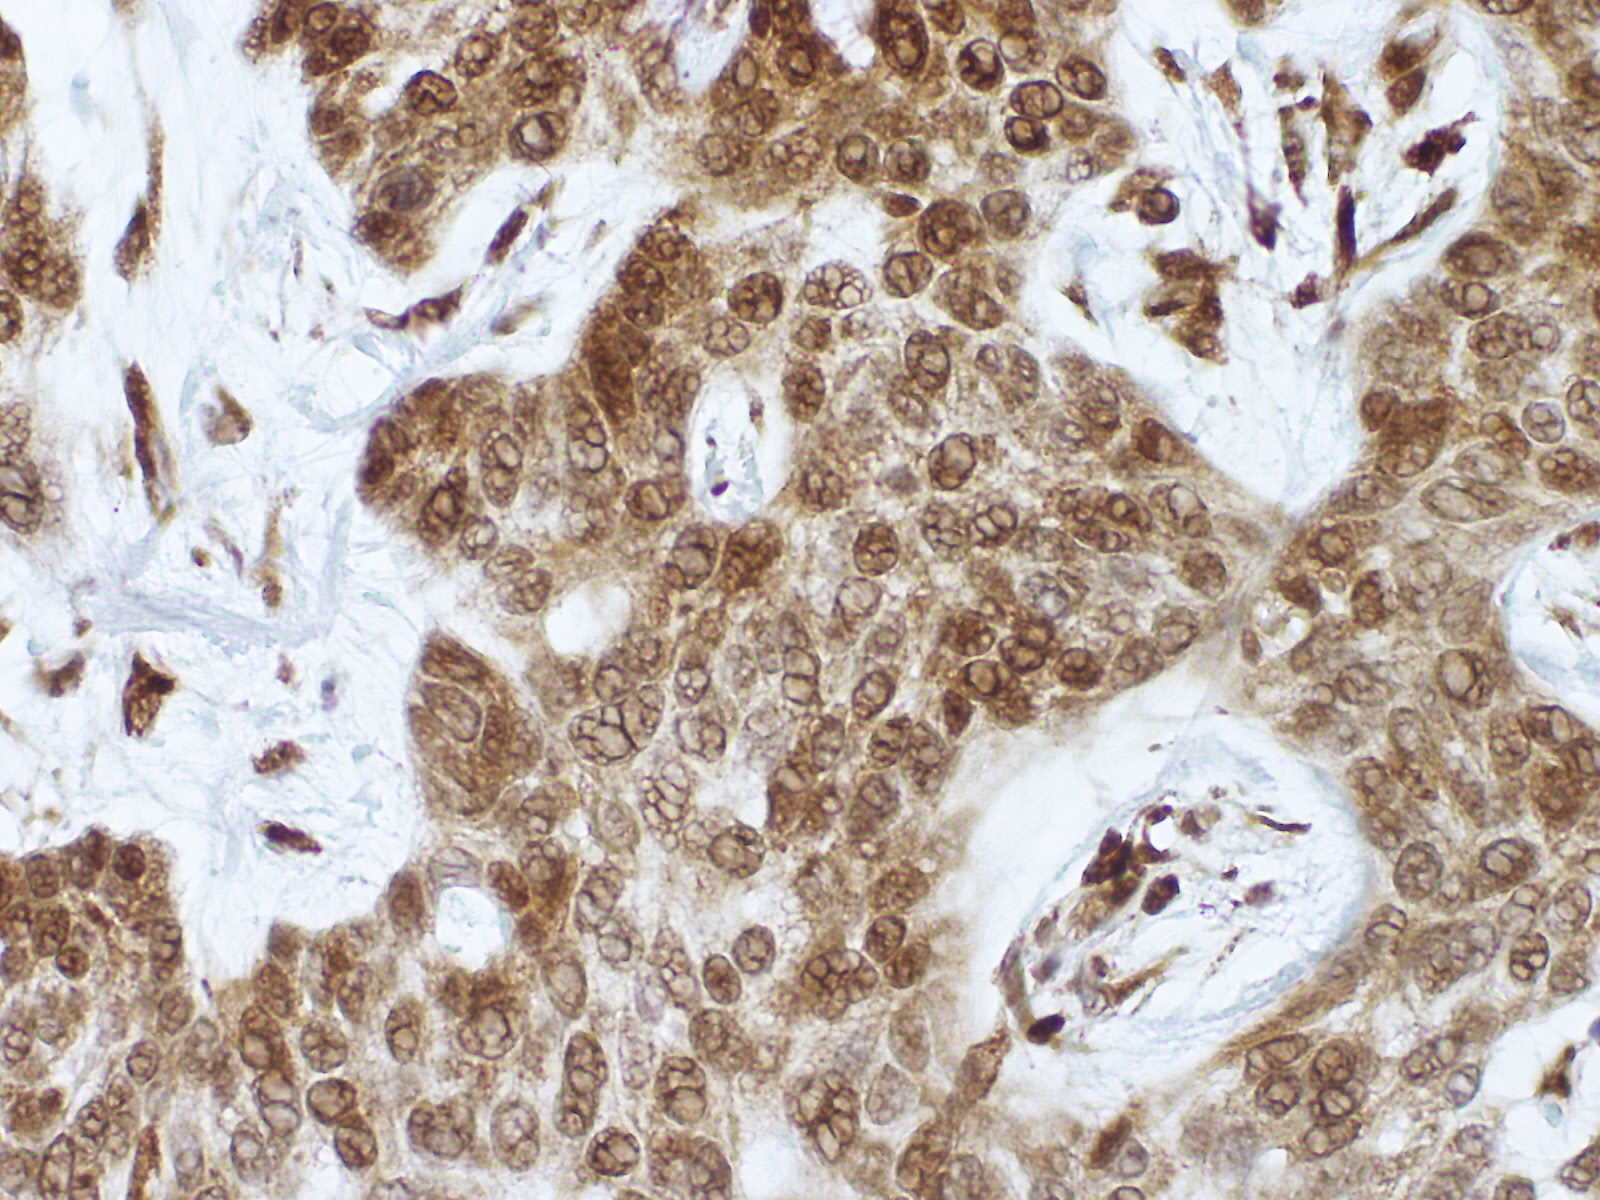
\includegraphics[width=\linewidth]{images/input.png}
        \caption{Obraz oryginalny}
    \end{subfigure}
    \begin{subfigure}{0.4\linewidth}
        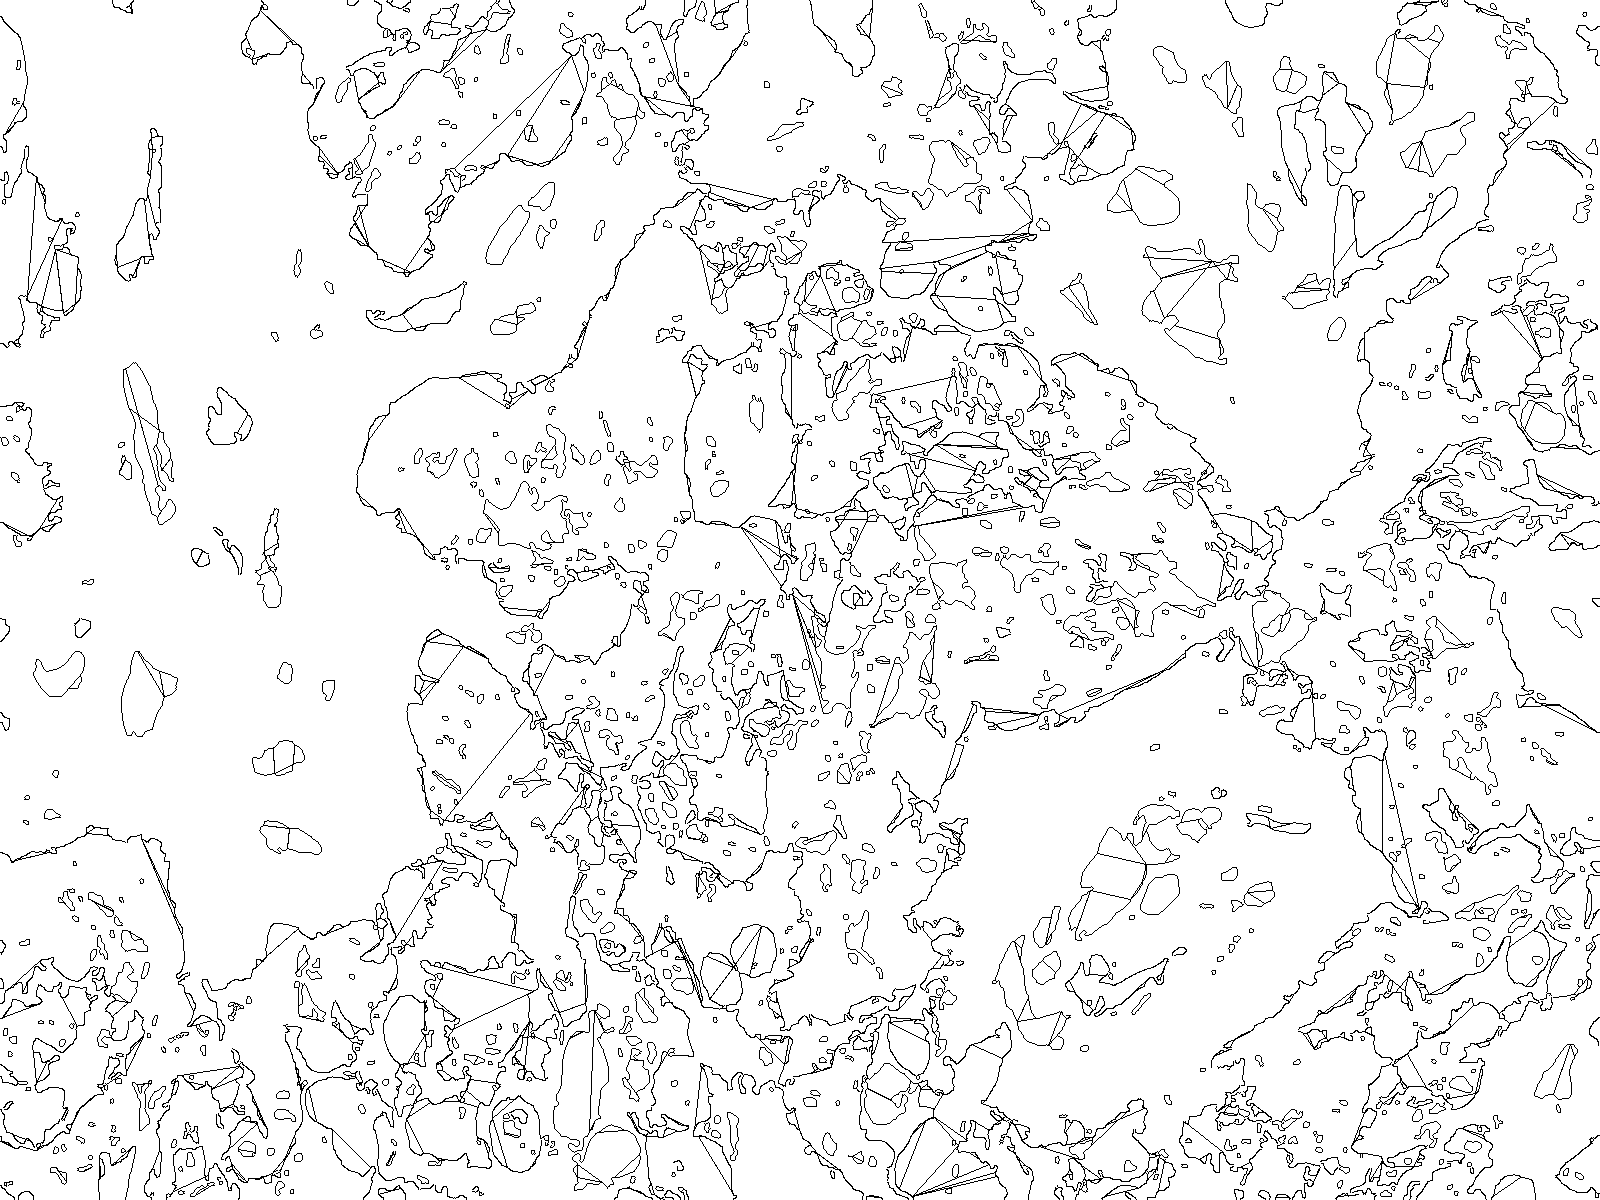
\includegraphics[width=\linewidth]{images/output.jpg}
        \caption{Lewy górny róg}
    \end{subfigure}
    \begin{subfigure}{0.4\linewidth}
        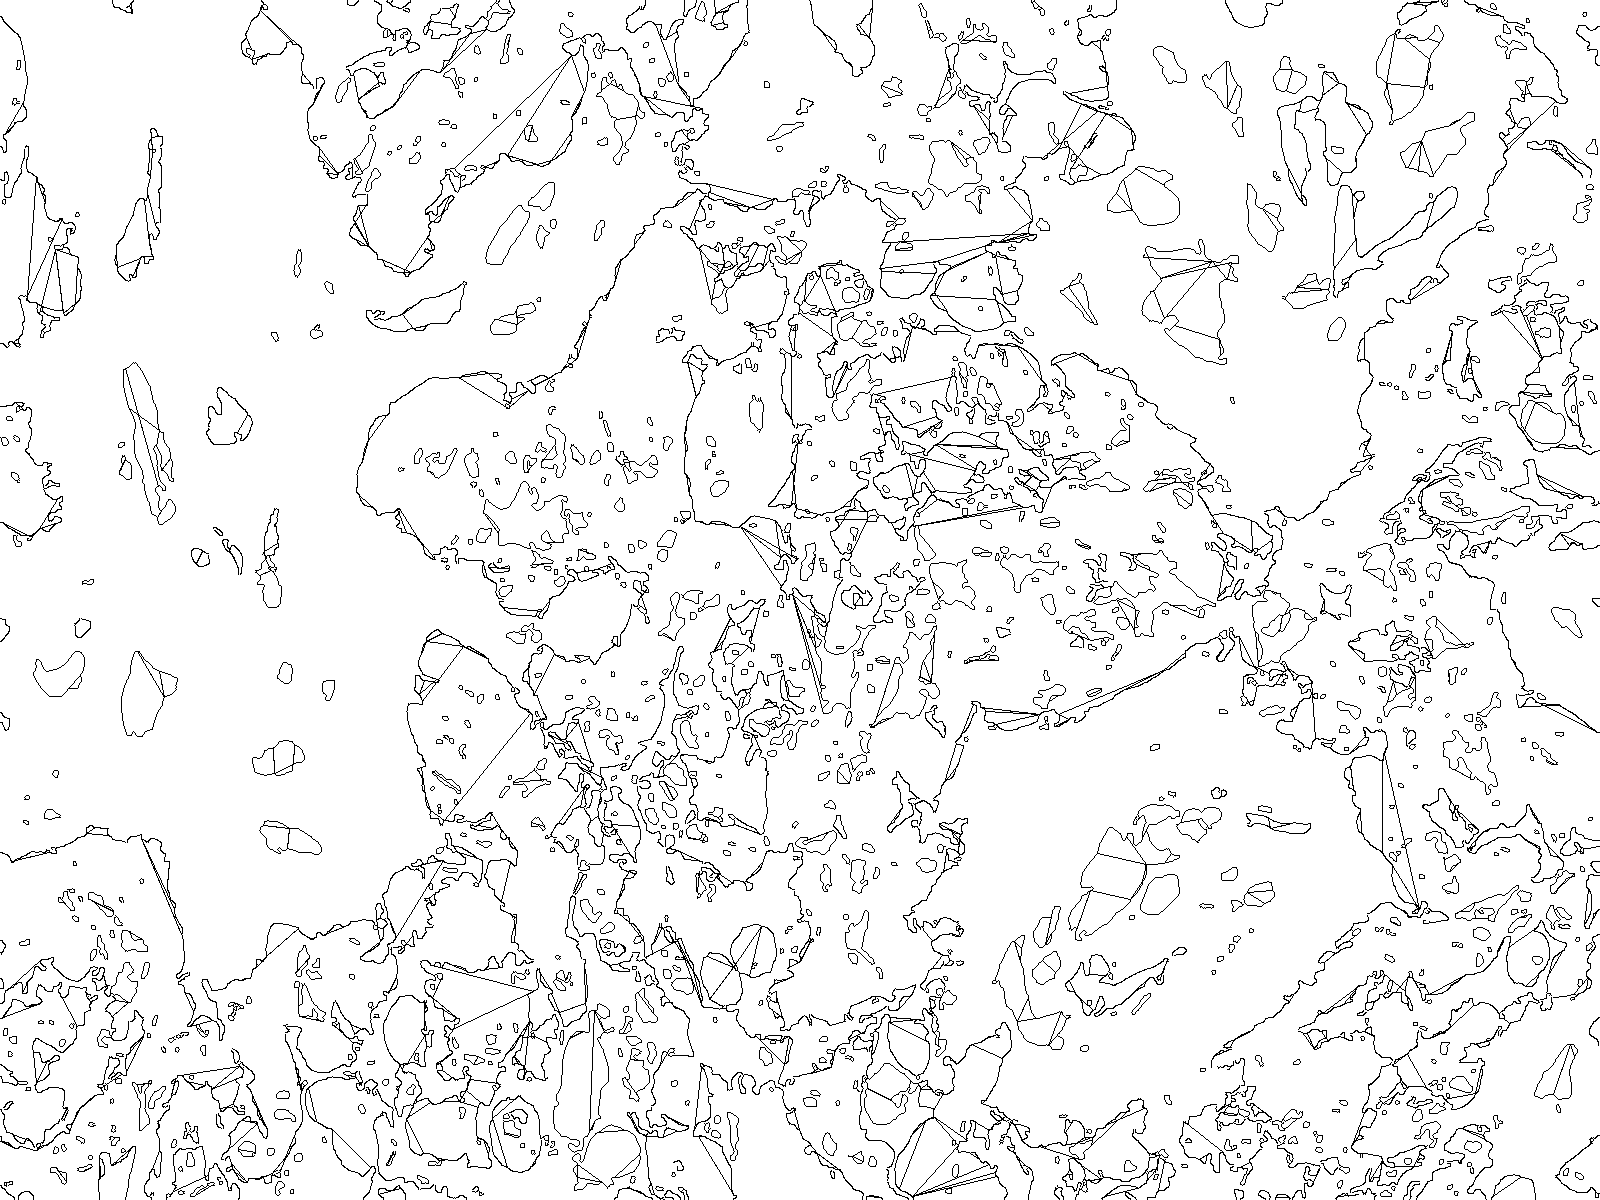
\includegraphics[width=\linewidth]{images/output.jpg}
        \caption{Kolejny obraz na prawo}
    \end{subfigure}
    \caption{Przykładowe cięcia obrazów wejściowych}
    \label{fig:input_split}
\end{figure}
Gdy model będzie już wyuczony w celu otrzymania segmentacji obraz wejściowy będzie najpierw dzielony w ten sam sposób, aby był zestawem mniejszych zdjęć, potem nastąpi segmentacja a po niej wyniki zostaną scalone ponownie w jeden obraz wyjściowy (w miejscach, gdzie będzie więcej niż jedna odpowiedź dla piksela z powodu kieszonki przyjmę wartość maksymalną).
Dzięki takiemu rozwiązaniu udało mi się znacząco zmniejszyć ilość pamięci operacyjnej wymaganej dla pojedyńczego przebiegu sieci, dzięki czemu mogę wykorzystać architekturę U-Net oraz znacząco zwiększyć jej skuteczność, ponieważ dostępną pamięć można wykorzystać by dodać dodatkowe warstwy/filtry.
Dodatkowo rozmiar 200 na 200 pikseli jest obrazem kwadratowym a z takimi najlepiej radzi sobię ta architektura.

Kolejnym plusem jest to, że w ten sposób ilość moich danych wejściowych drastycznie wzrośnie, ponieważ z każdego jednego obrazu utworzy się trzysta mniejszych, z których każdy będzie oddzielny/niezależnym przykładem uczącym (w tym wypadku obraz oryginalny składa się na siatkę o szerokości dwudziestu i wysokości piętnastu mniejszych obrazów).
Dzięki czemu otrzymujemy zamiast jednego przykładu uczącego trzysta.

Wprowadzając opisane powyżej podejście udało mi się uruchomić proces uczenia sieci neuronowej.
W wyniku otrzymałem jednak obraz który posiadał około 2 piksele czerwone, podczas gdy wszystkie pozostałe były czarne.
\subsubsection{Wybór jednego kanału - czerwony/alfa}
Analizując dane wyjściowe zauważyłem, że piksele tła posiadają wartości kanału alpha bliskie zeru natomiast piksele linii obrysowującej komórki przybierają wartości bliskie dwustu pięćdziesięciu pięciu.
Niemal identycznie wyglądały wartości kanału czerwonego.
Natomiast kanały zielony i niebieski miały niemal zawsze wartość równą zero.

Dlatego wpadłem na pomysł, żeby spróbować potraktować kanały alfa i czerwony jako obrazy monochromatyczne i użyć ich jako dane wyjściowe.
W ten sposób w założeniu predykcje tworzyłyby monochromatyczny obraz. W celu ujednolicenia wyników otrzymane tak obrazy zostały potraktowane jako kanał czerwony obrazu wynikowego a kanały niebieski i zielony otrzymały arbitralnie wartość zero dla wszystkich pikseli (otrzymany po takiej modyfikacji obraz był czarno/czerwony, tak jak oryginalne obrazy).
\begin{figure}[H]
    \centering
    \begin{subfigure}{0.4\linewidth}
        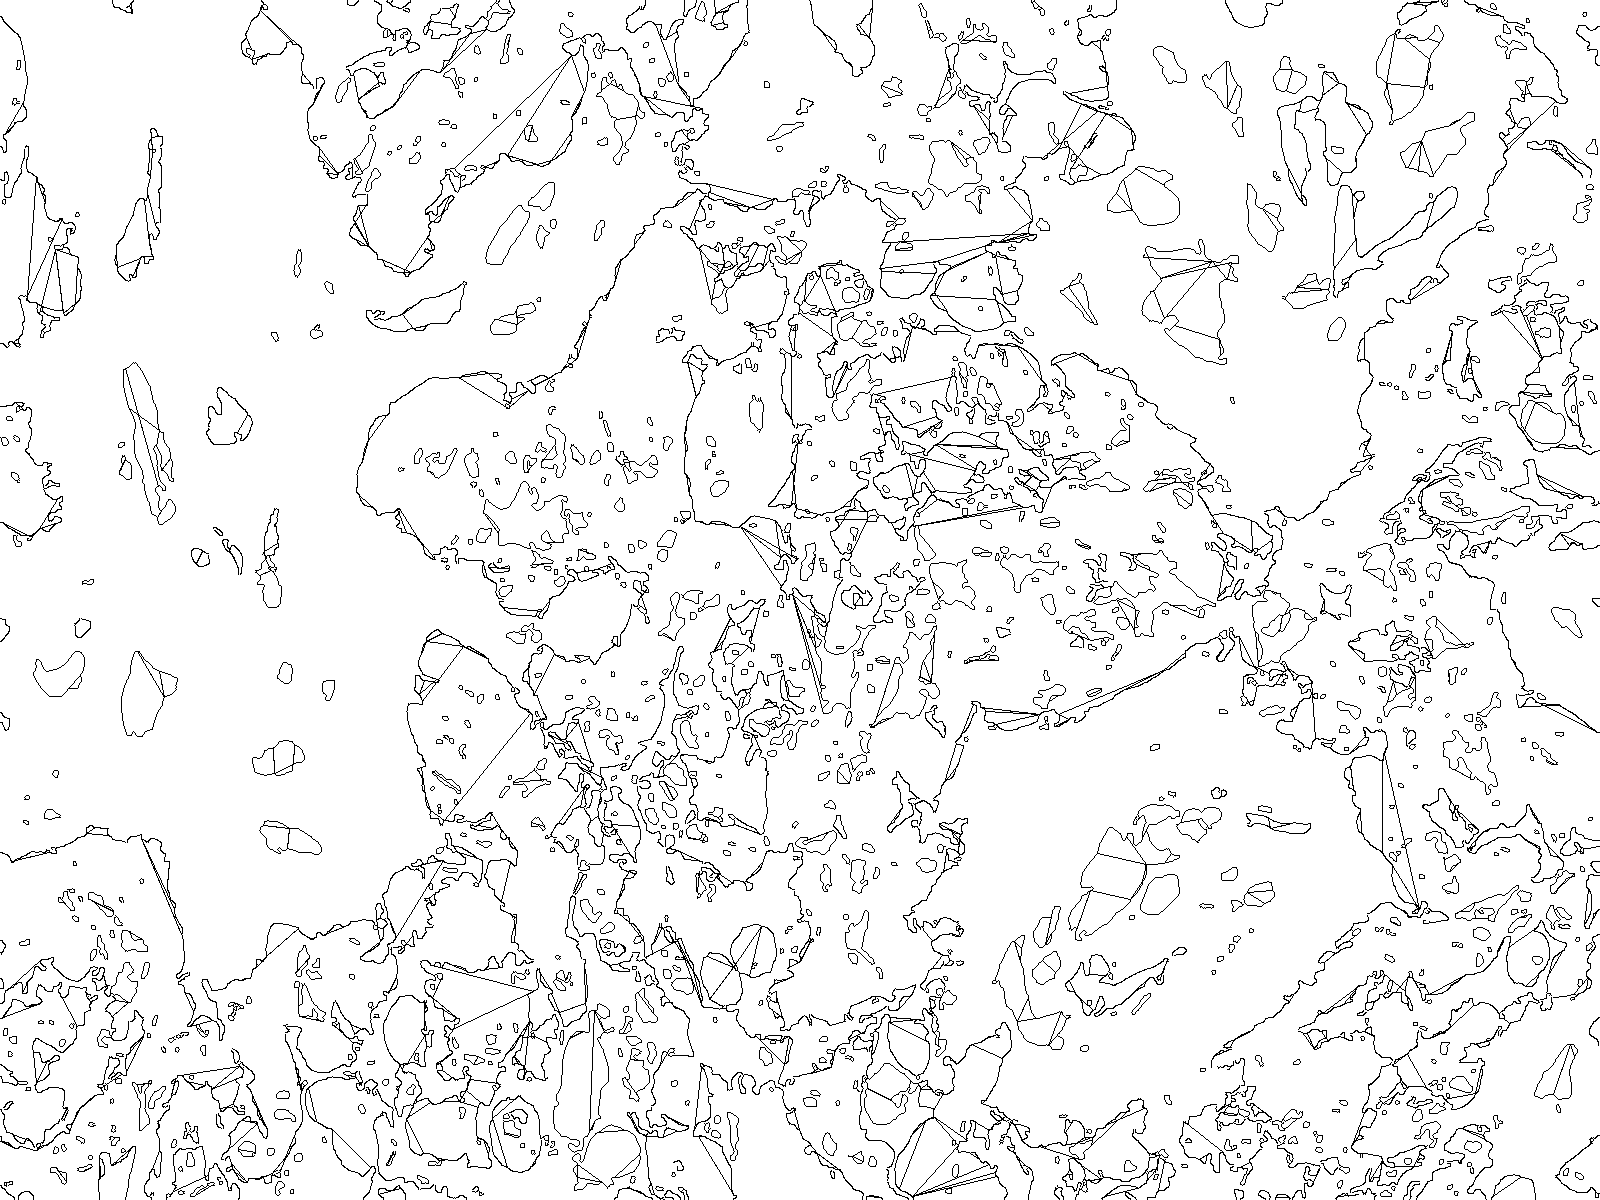
\includegraphics[width=\linewidth]{images/output.jpg}
        \caption{Lewy górny róg}
    \end{subfigure}
    \begin{subfigure}{0.4\linewidth}
        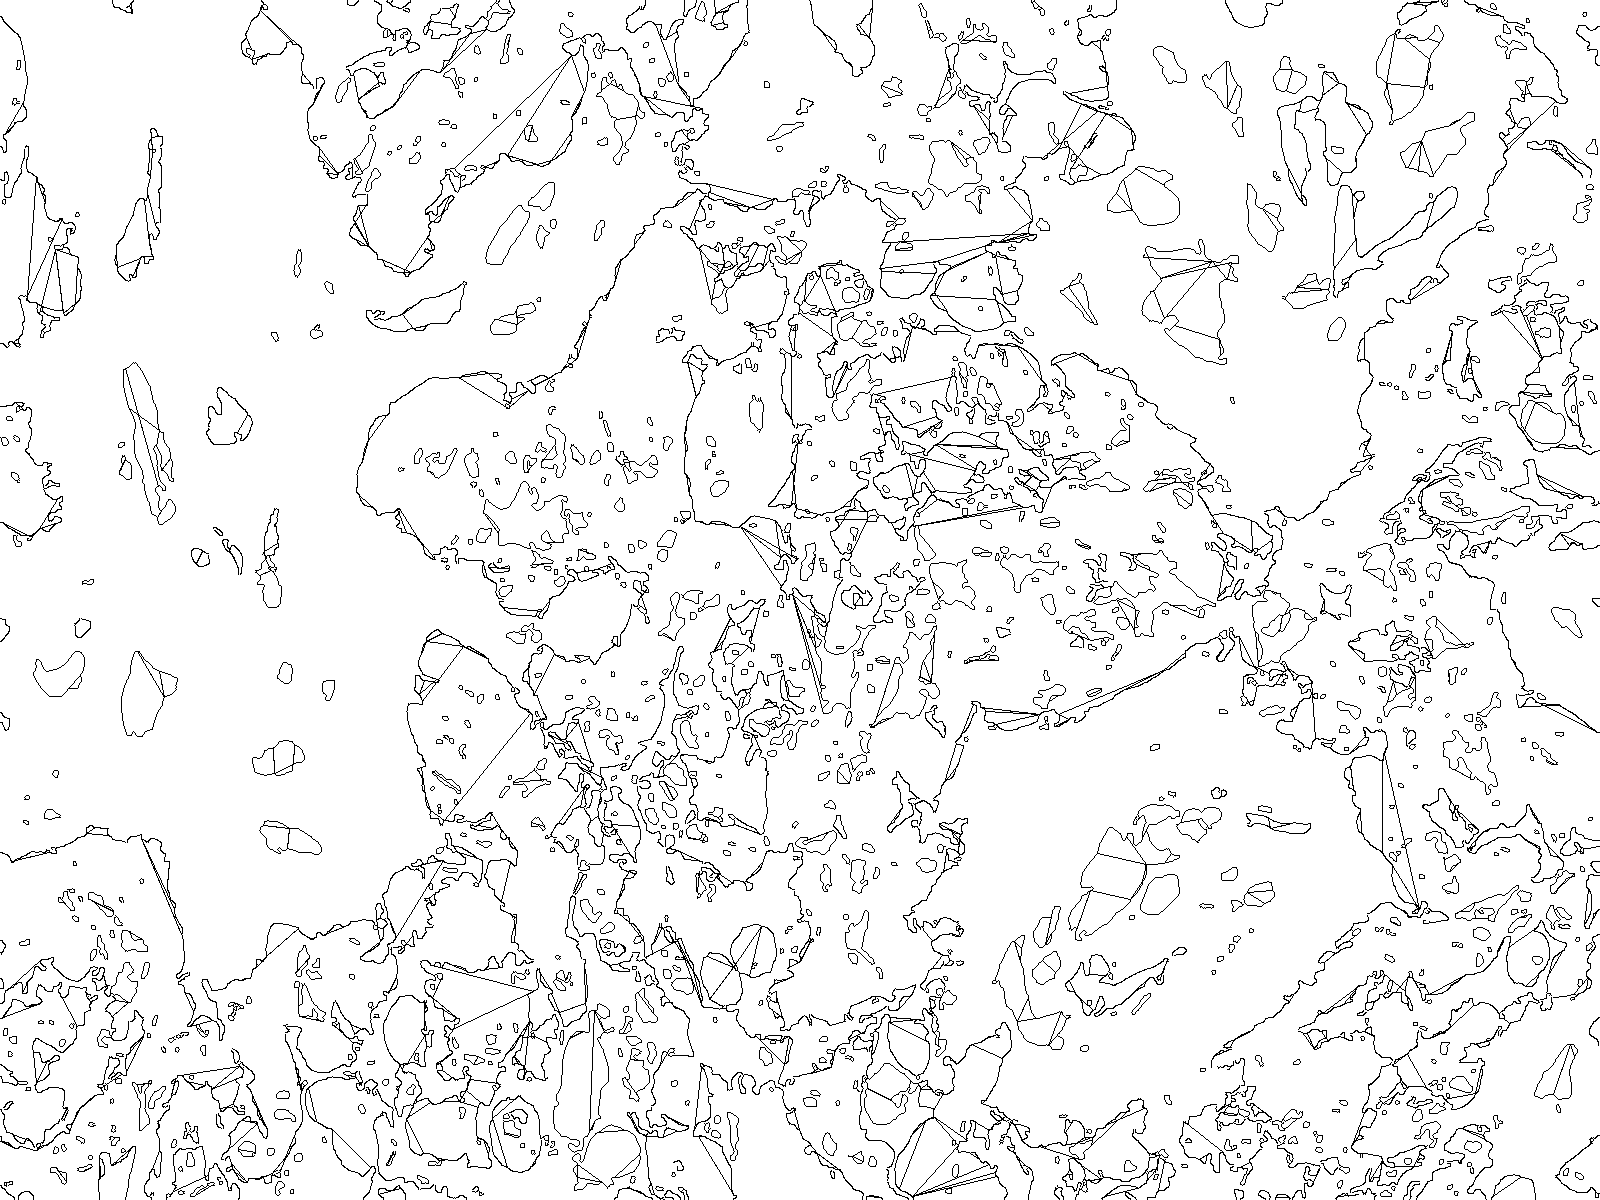
\includegraphics[width=\linewidth]{images/output.jpg}
        \caption{Kolejny obraz na prawo}
    \end{subfigure}
    \caption{Przykładowy otrzymany obraz}
    \label{fig:input_split}
\end{figure}

Niestety zastosowanie tego rozwiązania nie przyniosło porządnych efektów.
Obrazy wynikowe przyjmowały teraz w całości kolor czerwony (gdy jako wyjście przykładów uczących podaliśmy obraz monochromatyczny wygenerowany z kanału czerwonego) lub
czarny (gdy dane wyjściowe były na podstawie kanału alfa).
\subsubsection{Redukcja do obrazów trzy kanałowych i redukcja kolorów}
Kolejnym pomysłem było przeprowadzenie redukcję wymiarowości danych wyjściowych oraz zmniejszyłem ilość kolorów w obrazie.
Wartości kanałów czerwonego i alfa są ze sobą powiązane (dla tła obie zmierzają do zera).
Dlatego zdecydowałem się na zmianę obrazów wyjściowych z formatu RGBA do RGB.
Zależnie od wartości kanałów czerwonego i alfa zaokrągliłem kolor danego piksela do czystego czerwonego (255, 0, 0) lub czystego czarnego (0, 0, 0).
Przeprowadziłem te operację z różnymi wartościami progowymi dla obu kanałów.
W wyniku jednak nadal otrzymywałem całkowicie czerwone/czarne obrazy zależnie od tego jak dużo pikseli zostało zaokrąglonych do danego koloru.
\begin{figure}[H]
    \centering
    \begin{subfigure}{0.4\linewidth}
        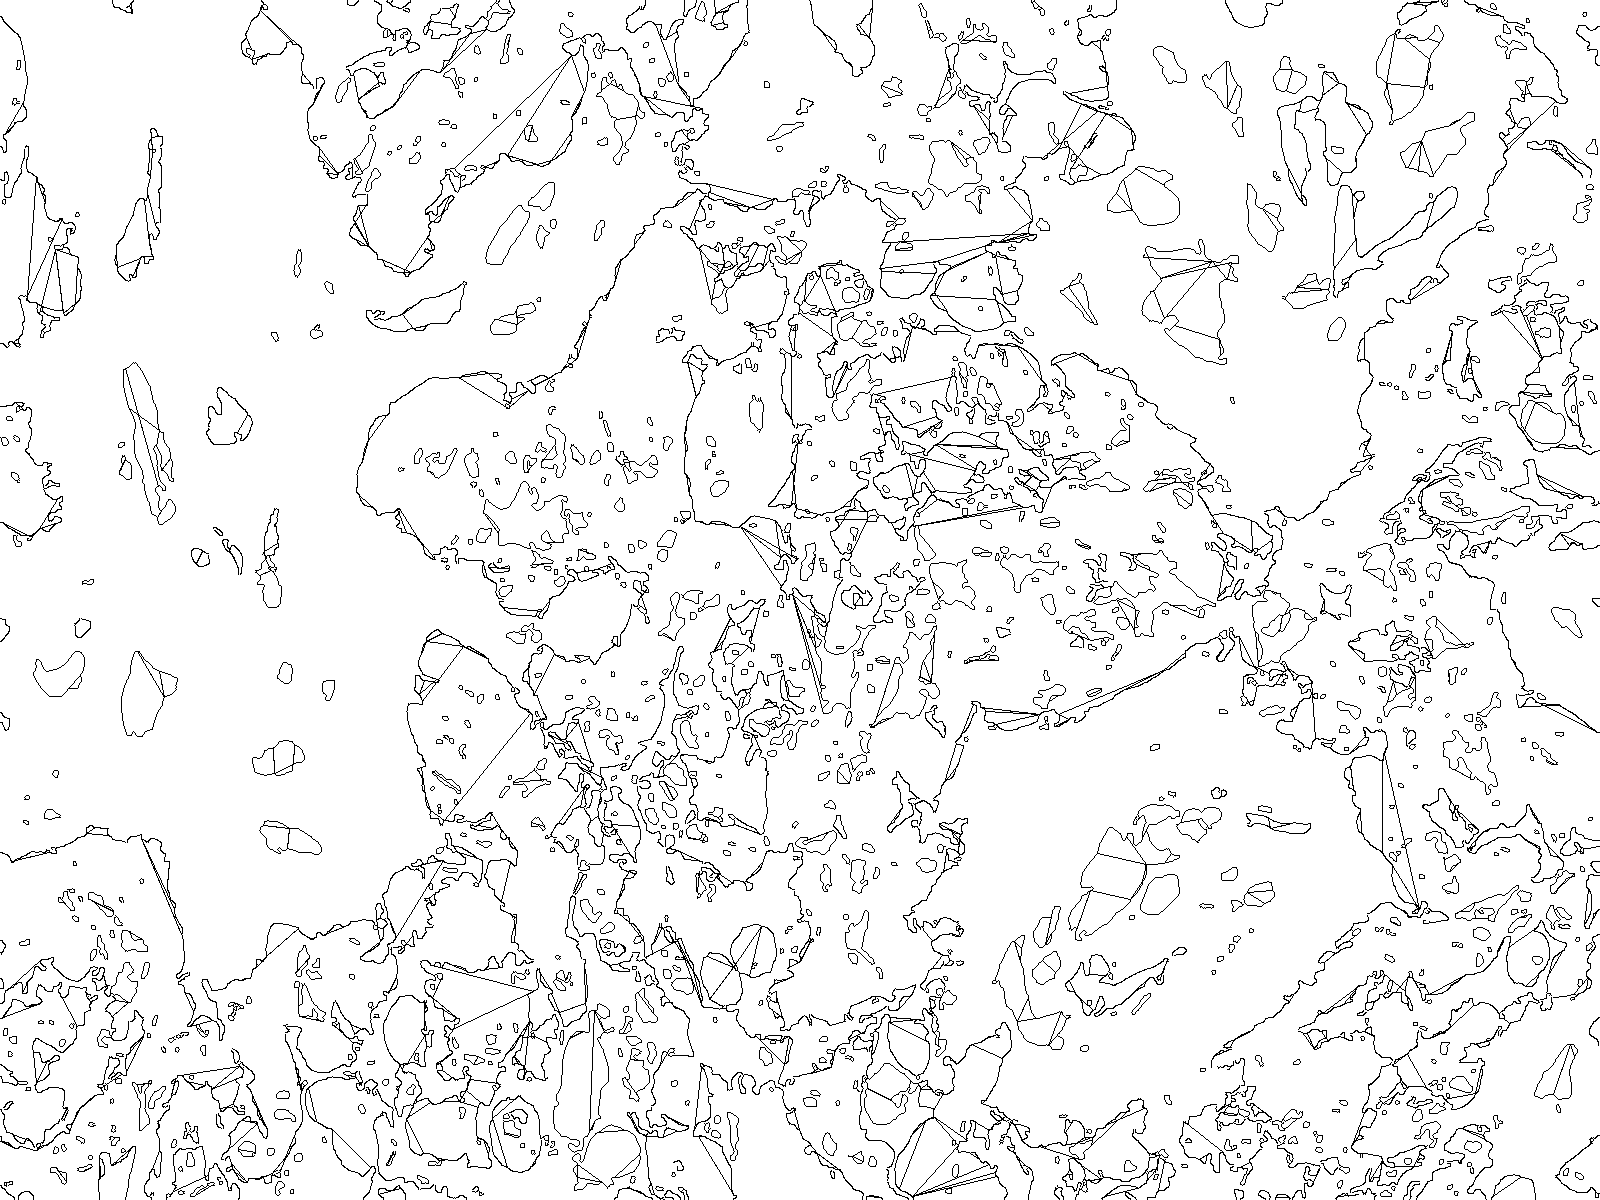
\includegraphics[width=\linewidth]{images/output.jpg}
        \caption{Lewy górny róg}
    \end{subfigure}
    \begin{subfigure}{0.4\linewidth}
        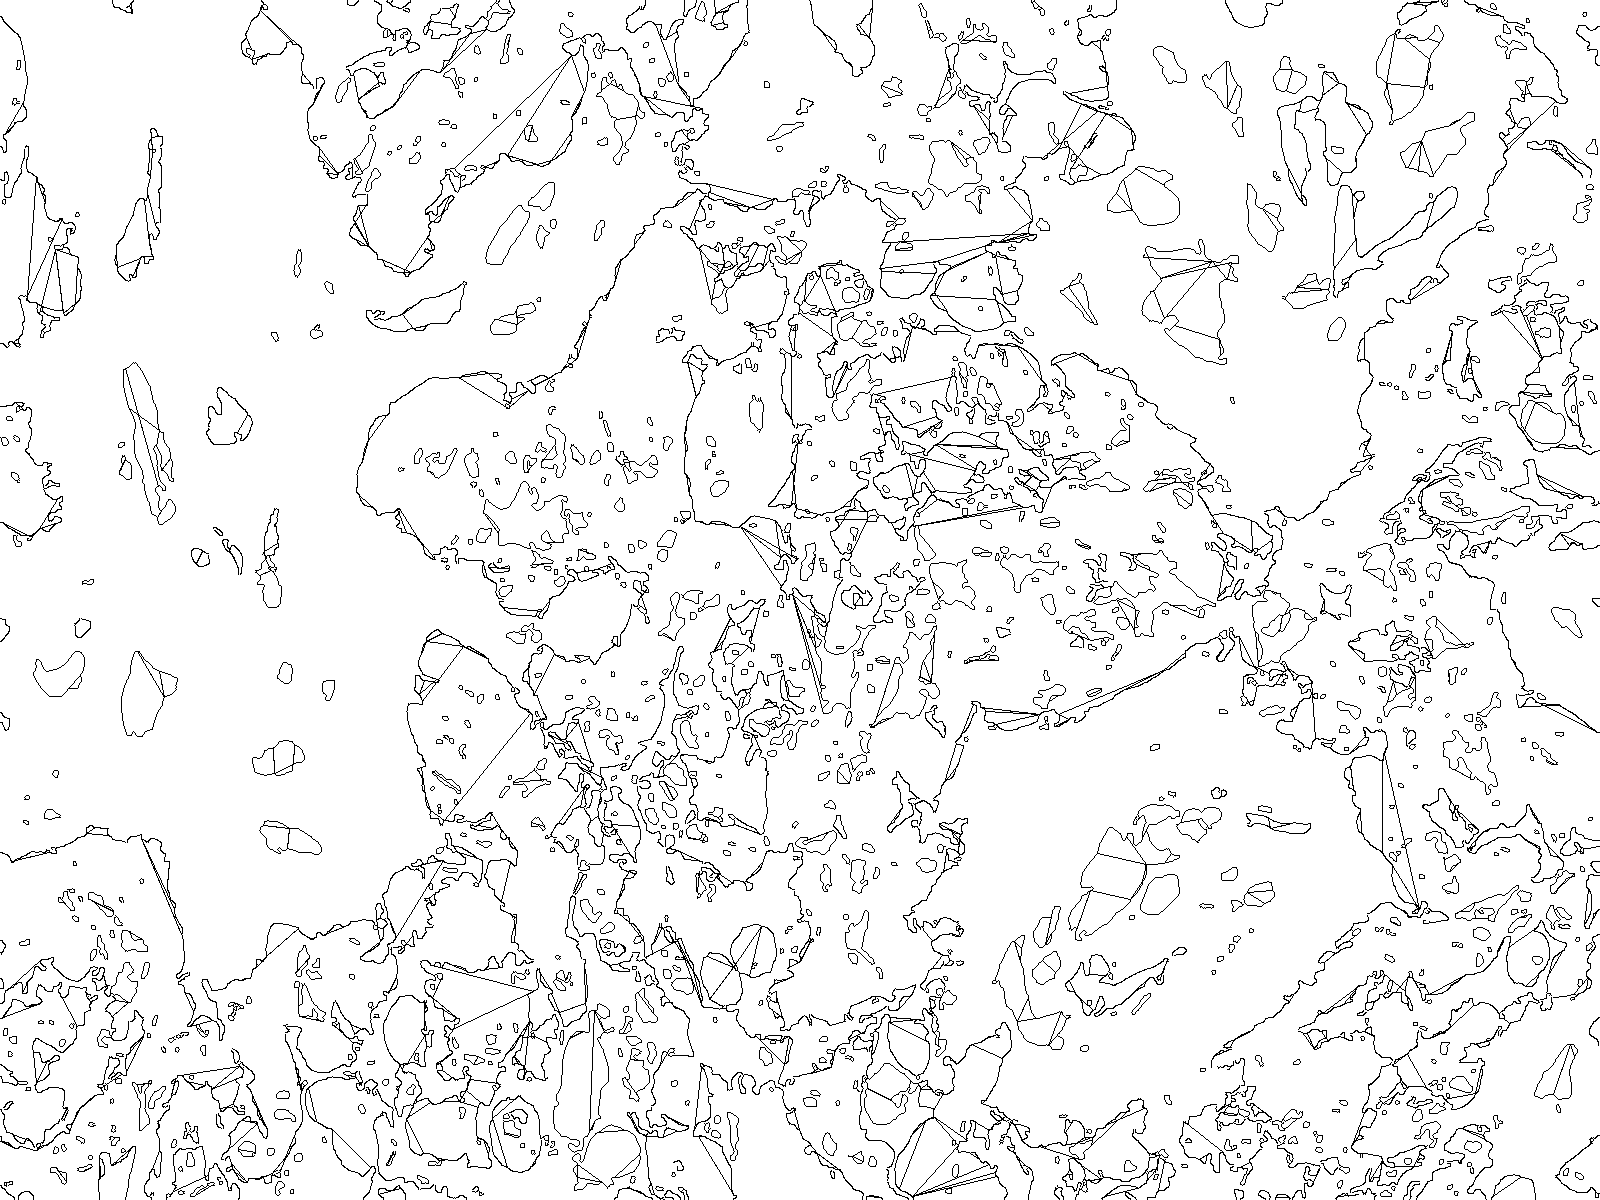
\includegraphics[width=\linewidth]{images/output.jpg}
        \caption{Kolejny obraz na prawo}
    \end{subfigure}
    \caption{Przykładowy otrzymany obraz}
    \label{fig:input_split}
\end{figure}

\subsubsection{Rozmycie Gausa}
Otrzymane w poprzednich próbach wyniki skłoniły mnie do myśli, że proporcje koloru czerwonego do czarnego są zbyt nierówne.
Z powodu tej nierówności model jest w stanie uzyskać wysoką wartość dokładności (rzędu dziewięćdziesięciu czterech procent) jako predykcję zwracając wszystkie piksele w tym samym kolorze.

Pomysłem na rozwiązanie tego problemu było zastosowanie na obrazach docelowych rozmycia Gaussa przed pokazaniem ich sieci.
Filtr ten rozmywa obraz co w wypadku dwu kolorowego obrazu zawierającego linie oraz tło będzie skutkowało poszerzeniem linii.
\begin{figure}[H]
    \centering
    \begin{subfigure}{0.4\linewidth}
        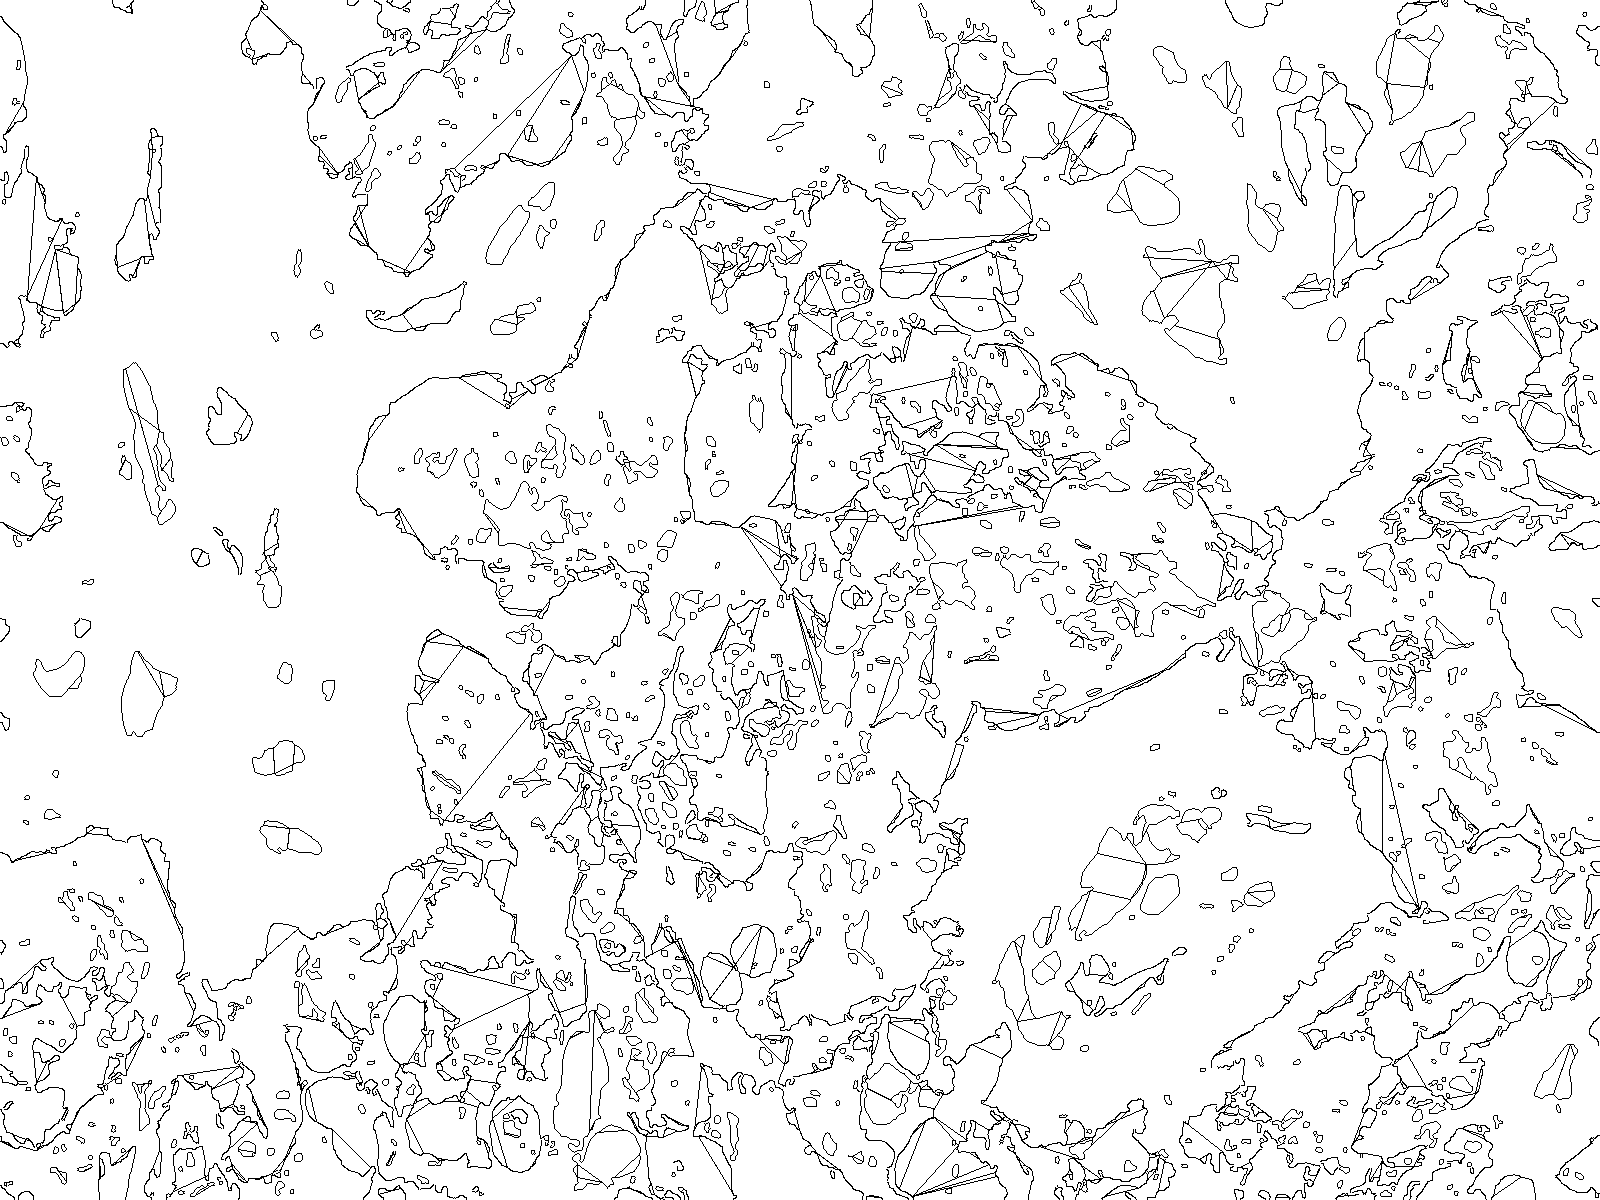
\includegraphics[width=\linewidth]{images/output.jpg}
        \caption{Przed}
    \end{subfigure}
    \begin{subfigure}{0.4\linewidth}
        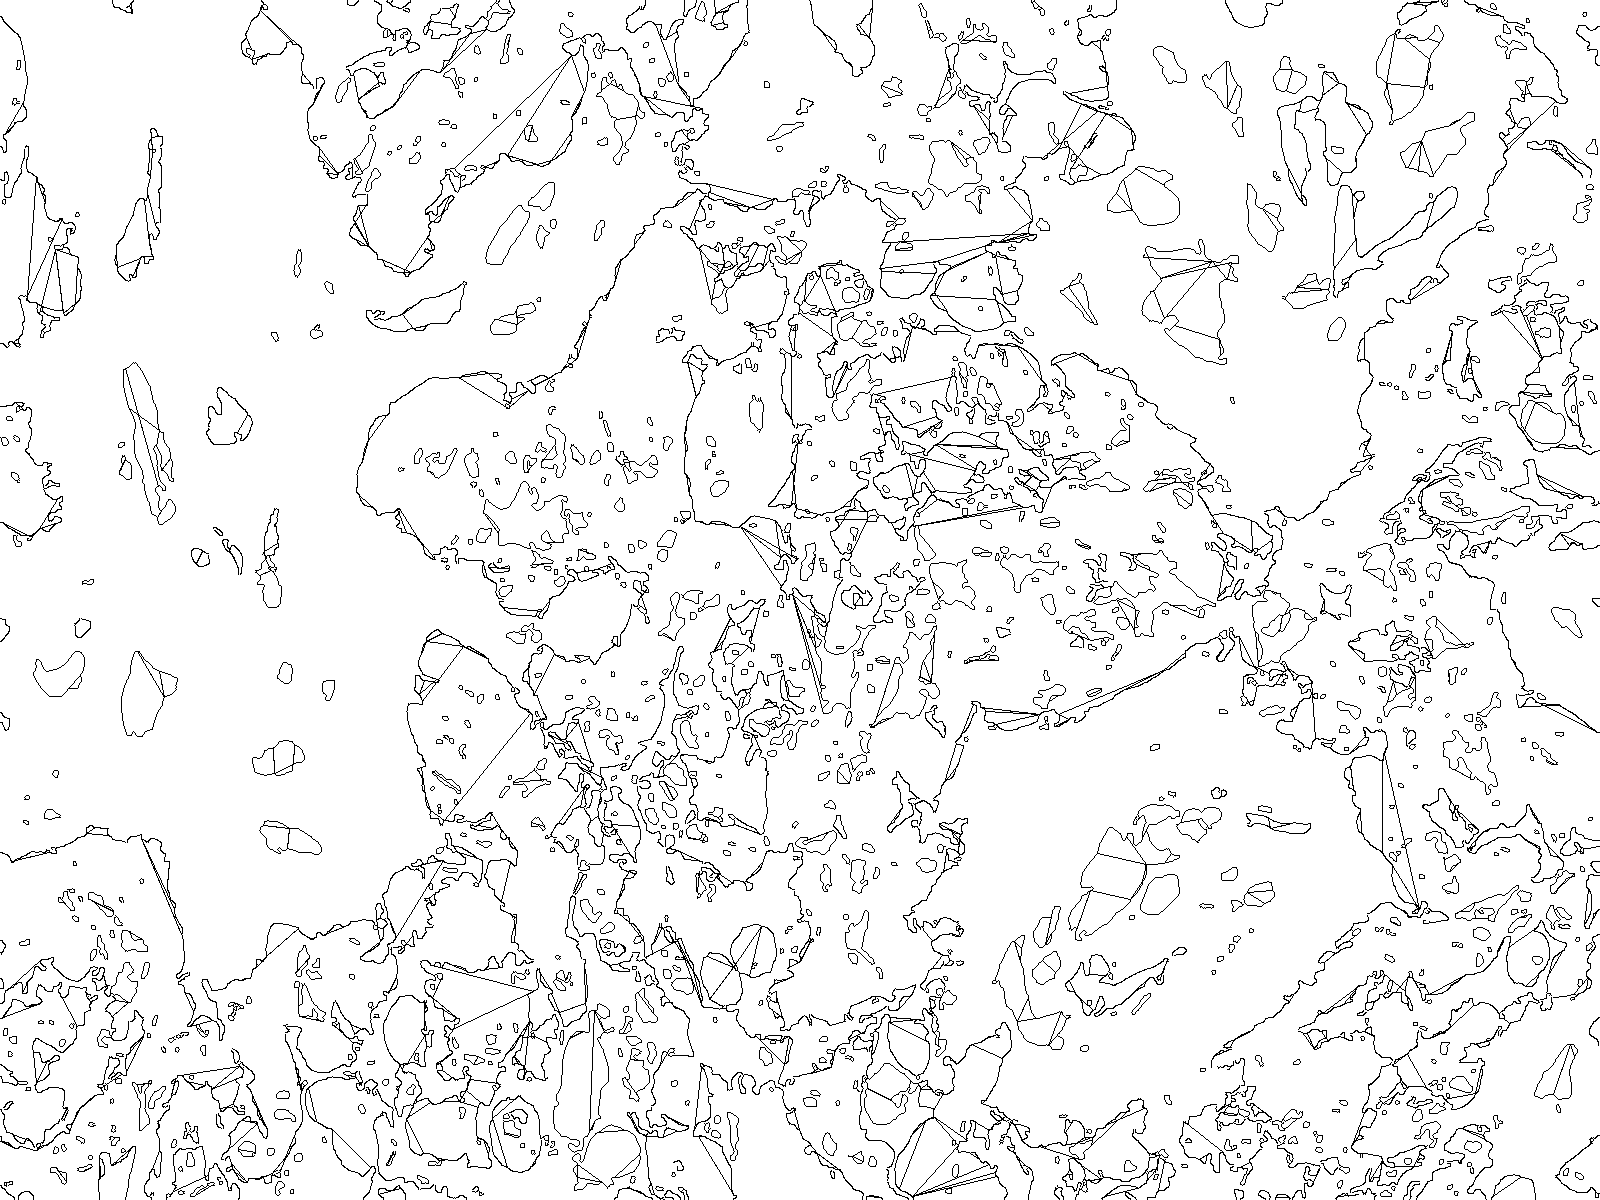
\includegraphics[width=\linewidth]{images/output.jpg}
        \caption{Po}
    \end{subfigure}
    \caption{Obraz wyjściowy przed i po zastosowaniu filtra}
    \label{fig:input_split}
\end{figure}
\subsection{Funkcje start}
We wszystkich wykonanych do tej pory eksperymentach otrzymywałem jako predykcję jednokolorowe obrazy.
Jednakże dla każdego z tych podejść otrzymywałem bardzo wysoką wartość dokładności i małą wartość funkcji strat.
Dlatego zdecydowałem się na zbadanie innych sposobów oceny poprawności działania sieci.
\subsubsection{Funkcja strat - Współczynnik Sørensena}
Często używaną w zagadnieniu segmentacji funkcją strat jest $1-QS$ gdzie QS to współczynnik Sørensena opisany wzorem:
\begin{equation}
    QS = \frac{2*|X \cap Y|}{|X|+|Y|}
\end{equation}
Dla:
\begin{itemize}
    \item X - zbiór wejściowy
    \item Y - zbiór wyjściowy
\end{itemize}

\begin{lstlisting}[caption={Implementacja przy użyciu Keras i TensorFlow}]
from tensorflow.keras import backend as K

def custom_metric(y_true, y_pred):
    y_true = K.flatten(y_true)
    y_pred = K.flatten(y_pred)
    return (2. * K.sum(y_true * y_pred) +1) / (K.sum(y_true) + K.sum(y_pred) + 1)
\end{lstlisting}

Korzystając z tej funkcji strat otrzymałem prawie dokładnie takie same obrazy wyjściowe.
Jednakże w przeciwieństwie do użycia dokładności jako metryki otrzymane wartości oscylowały w okolicy dwudziestu procent (zamiast okolic dziewięćdziesięciu procent).

\subsubsection{Własna funkcja strat}
Kolejny pomysł opierał się na tym aby metryka mierząca poprawność zwracała większą uwagę na poprawnie sklasyfikowane czerwone piksele (gdyż jest ich znacznie mniej).
Piksele, które zostaną poprawnie z kategoryzowane a mają kolor czerwony będą ``X`` razy ważniejsze niż poprawnie sklasyfikowane piksele czarne.

\begin{align}
    \frac{X*\frac{PC}{AC} + \frac{PCZ}{ACZ}}{x+1}
\end{align}

Gdzie:
\begin{itemize}
    \item X - waga ile razy ważniejsze są piksele czerwone
    \item PC - liczba poprawnie sklasyfikowanych czerwone pikseli
    \item AC - liczba wszystkich czerwonych pikseli
    \item PCZ - liczba poprawnie sklasyfikowanych czarnych pikseli
    \item ACZ - liczba wszystkich czarnych pikseli
\end{itemize}

\subsection{Obliczenie predykcji na komputerze klienckim}
Jednym z problemów przy pracy z danymi medycznymi jest to, że nie mogą one opuścić sieci wewnętrznej szpitala.
Dlatego nie możemy uruchomić wytrenowanego modelu na serwerze i zapewnić możliwości odpytania poprzez API.

Rozwiązaniem w tej sytuacji było przeniesienie wytrenowanych w TensorFlow modeli do TensorFlowJS który pozwala na użycie ich na komputerze klienckim.
Testy te były dokonane na znacznie prostszy modelu służącym do rozpoznawania odręcznie pisanych cyfr ze zbioru MNIST (stosował on jednak wszystkie warstwy z, których składa się model w architekturze U-Net, jedynie w innej ilości/konfiguracji).

Pierwszym krokiem było przekształcenie modelu z biblioteki Python-owej na bibliotekę javascript-ową.
Można to było łatwo wykonać w skrypcie Python-owym za pomocą metody tfjs.converters.save\_keras\_model, której przekazujemy model oraz ścieżkę do niego.
Największym problemem w tej zmianie było jednak to, że aby użyć biblioteki w javascript operacje przez nią wykonywane musiały być poza wątkiem głównym, w celu nie blokowania UI - jest to narzucane przez samą bibliotekę.
Aby to osiągnąć posłużyłem się tak zwanymi webworker-ami.
Pozwalają one na wykonywanie zadań równolegle do wątku głównego.
W wątku głównym tworzymy obiekt klasy Worker oraz subskrybujemy wydarzenie worker.onmessage.
Dzięki temu możemy wykonać operację na danych otrzymanych w wiadomości. Natomiast w celu wysłania zapytania do workera używamy metody worker.postMessgae w której przekazujemy dane.
W moim wypadku była to pobrana z wyświetlonej kanwy tablica z danymi o pikselach w obrazku.
W skrypcie zawierającym kod źródłowy workera również subskrybujemy wydarzenie onmessage, w jego obsłudze najpierw preprocesuję dane w ten sposób aby ich format na wejście był taki sam jak danych uczących.
Jest to wymagane nawet jeżeli chcielibyśmy sprawdzić model korzystając z tego samego obrazu ponieważ biblioteki PIL oraz NumPy mają inny format danych niż dane zwrócone przy pomocy javascript z obiektu canvas dostępnego w HTML5 na którym wyświetlany był obraz do klasyfikacji.
Następnie po doprowadzeniu otrzymanych danych do odpowiedniego formatu jesteśmy w stanie użyć wyuczonego w Pythonie i TensorFlow modelu w celu uzyskania predykcji.
Następnie za pomocą metody postMessage jesteśmy w stanie wysłać do wątku głównego wiadomość zawierającą predykcję modelu, który ją wyświetli.

Dzięki powyższemu rozwiązaniu jesteśmy w stanie uruchomić nasz model po stronie klienta w przeglądarce.
Dodatkowo zapewniona jest płynność działania ponieważ procesowanie danych oraz predykcja modelu wykonywane są równolegle do wątku głównego, który obsługuje interfejs użytkownika.

\begin{figure}[H]
    \centering
    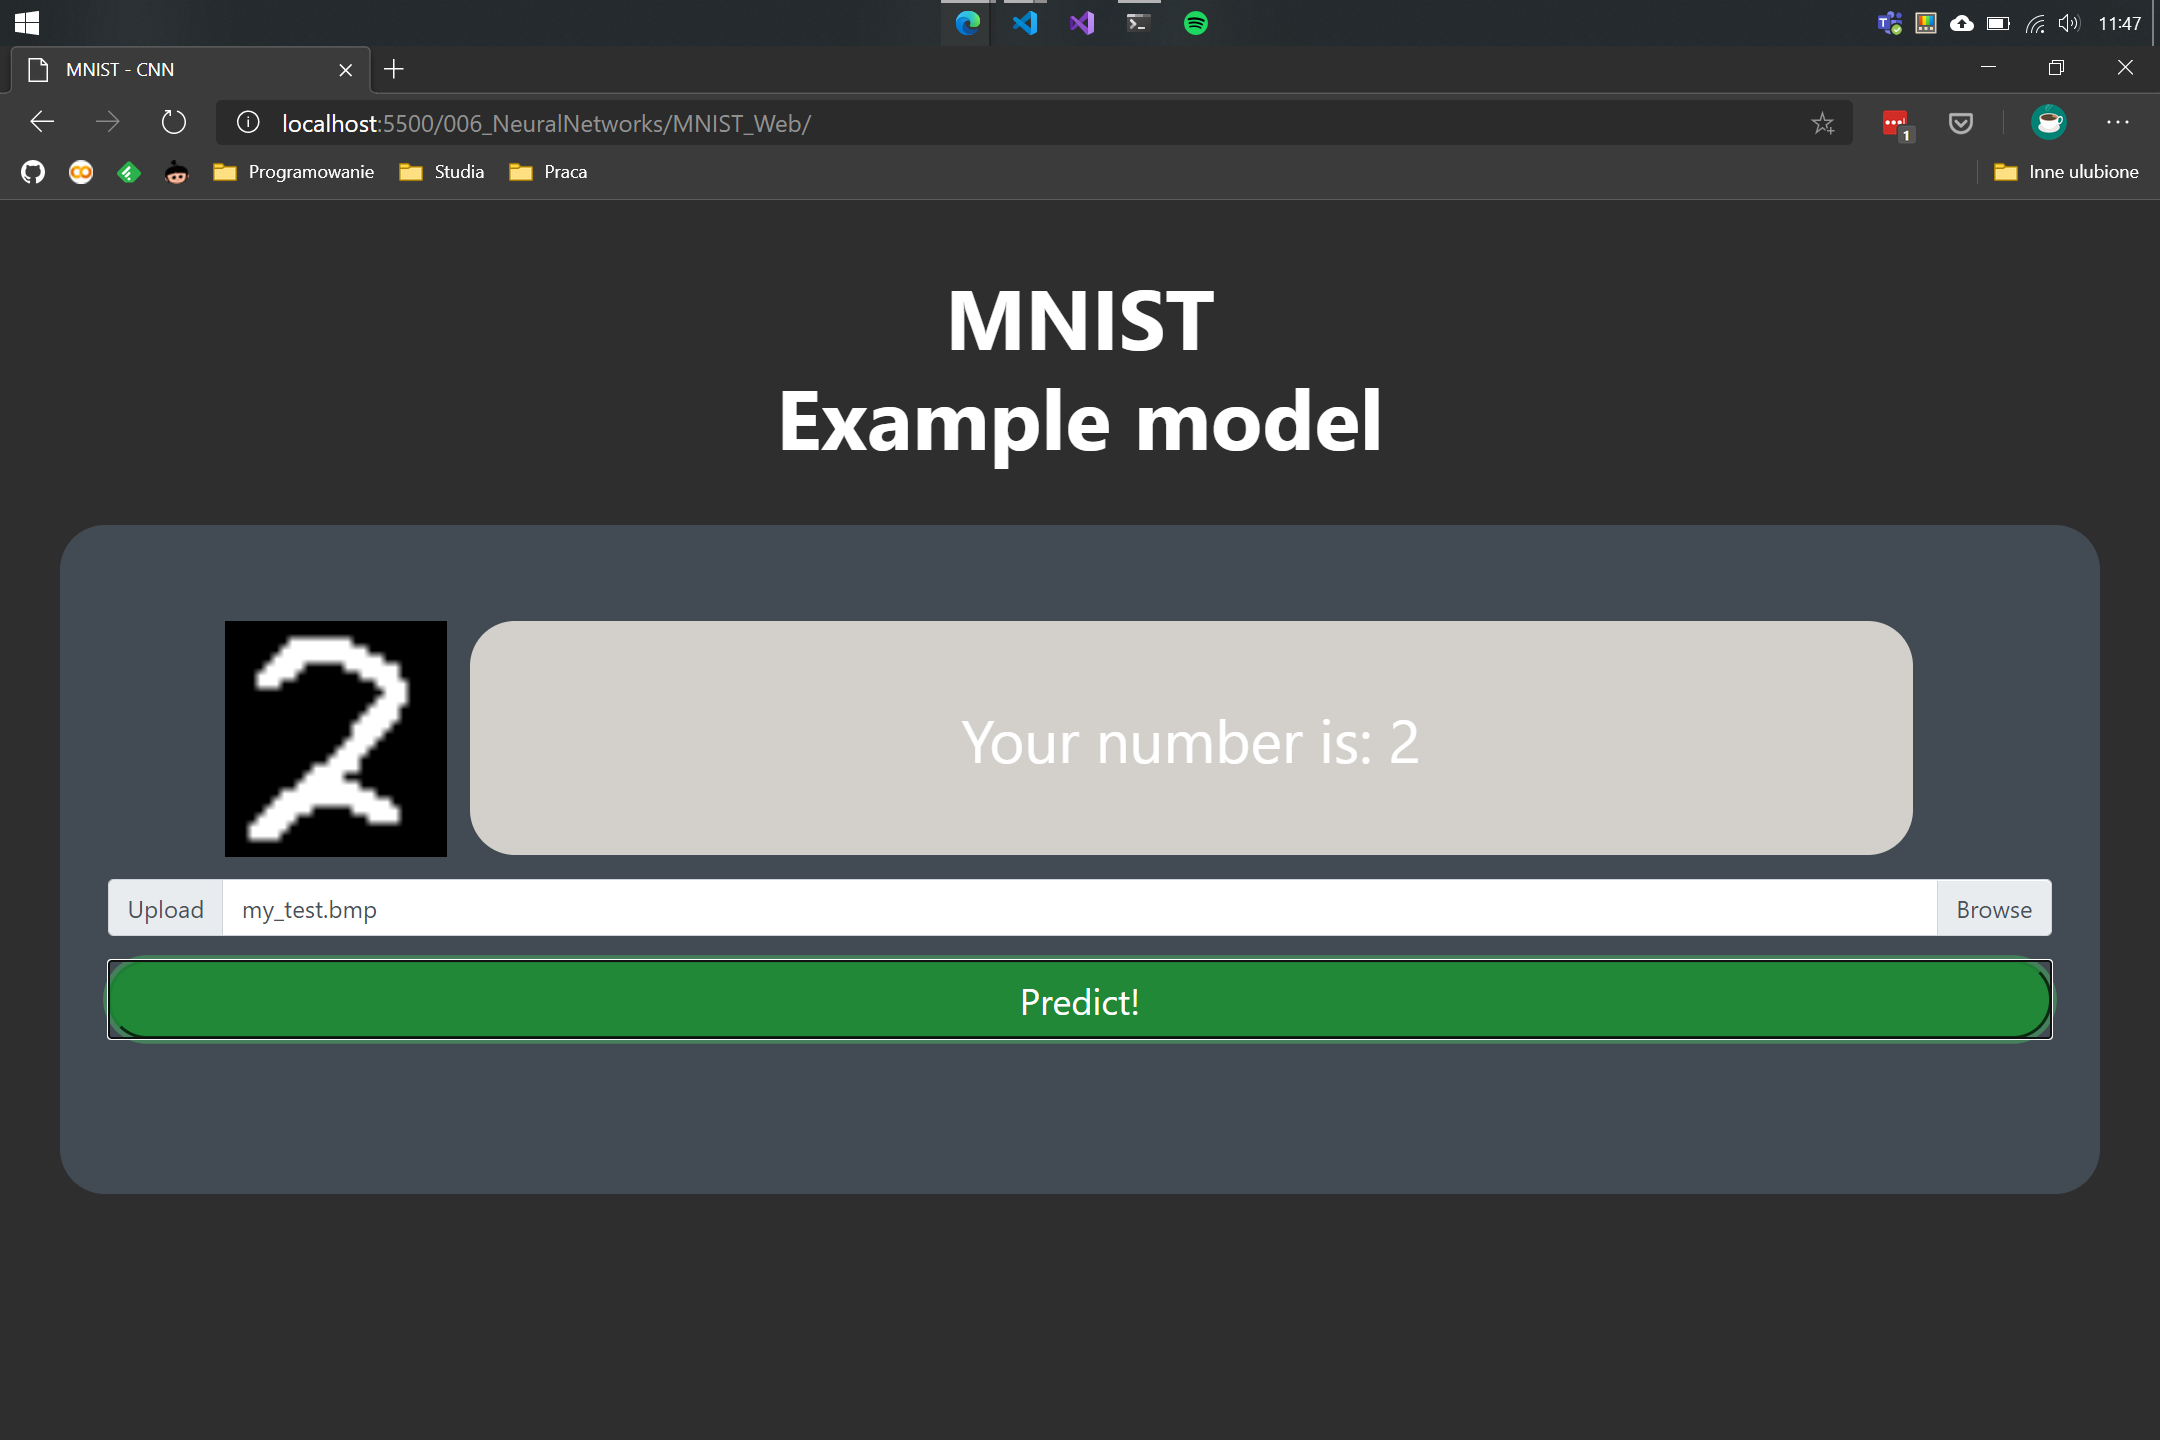
\includegraphics[width=\linewidth]{images/mnist.png}
    \caption{Przykład klasyfikacji obrazu w przeglądarce}
    \label{fig:mnist}
\end{figure}
\newpage
\section{Powstałe narzędzia}
W trakcie prac powstał szereg narzędzi mających za zadanie ułatwić pracę nad tym zagadnieniem.
Kod wraz z historią jest dostępny na platformie GitHub\footnote{https://github.com/mtracewicz/CellSegmentation}.
Wyniki są prezentowane za pomocą platformy GitHub Pages\footnote{https://mtracewicz.ksummarized.com/CellSegmentation/}.
\subsection{Skrypty pozwalające na preprocessing obrazów uczących}
W ramach prac stworzyłem cztery skrypty pozwalające na edycję zdjęć wejściowych/wyjściowych.
Powstałe skrypty pozwalają na:
\begin{itemize}
    \item zastosowanie filtra rozmycia Gaussa z wybranym parametrem na pojedyńczym obrazie lub katalogu obrazów
    \item pocięcie obrazów na mniejsze nachodzące się na siebie obrazki
    \item zespolenie obrazków utworzonych poprzednim skryptem z powrotem w całość
    \item zredukowanie kanałów obrazów z RGBA do RGB i zaokrąglenie wartości pikseli do czerwonego (255, 0, 0) i czarnego (0, 0, 0)
\end{itemize}
\subsection{Skrypt do uczenie sieci}
W celu umożliwienia automatyzacji procesu uczenia stworzyłem skrypt pozwalający na uruchamiane procesu uczenia z różnymi parametrami.
Dzięki takiemu podejściu jesteśmy przykładowo w stanie uruchomić przez noc proces uczenia dla kilku różnych kombinacji architektur, hiperparametrów, danych wejściowych/wyjściowych.

Skrypt przyjmuje na wejściu pod jaką nazwą ma zostać zapisany wytrenowany model oraz katalogi ze zdjęciami wejściowymi i wyjściowymi.

Dodatkowo opcjonalnie możemy podać ścieżkę do skryptu napisanego w języku Python w, którym znajdują się funkcje o nazwach ``custom\_loss`` i ``custom\_metrics`` (w wypadku braku domyślnie użyty jest współczynnik Sørensena), które zostaną użyte jako metryka oraz funkcja strat.

Kolejnym opcjonalny parametr jest odpowiedzialny za użytą architekturę, jest to ścieżka do pliku zawierającego funkcję ``get\_model``, która zwraca obiekt klasy ``tf.Keras.Model`` (domyślnie używany jest model z moją implementacją architektury U-Net).

Następny parametr to ścieżka do pliku zawierającego hiperparametry jako zmienne w skrypcie języka Python (domyślnie jest to plik ``hyperparameters.py`` z napisanego przeze mnie moduły ``neural\_network``).

Skrypt zaczyta dane do pamięci a następnie wykona uczenie modelu (``tf.keras.Model.fit'') na podanych danych ze wskazaną funkcją strat, metryką, hiperparametrami i architekturą.
Następnie wynikowy model zostanie zapisany pod wskazaną nazwą w katalogu ``trained\_models``.
\subsection{Skrypt pozwalające na testowanie zapisanych modeli}
Kolejny skrypt przyjmuje na wejście ścieżkę do zapisanego modelu oraz ścieżki do katalogów zawierających dane wejściowe i wyjściowe.
A następnie przeprowadza na nich test sprawdzający jak dobrze model sobie na nich poradził za pomocą metody model.evaluate.
\subsection{Skrypt pozwalające na predykcję dla obrazu/folderu obrazów}
Stworzyłem również skrypt, który otrzymując na wejście ścieżkę do modelu, którego chcemy użyć oraz
ścieżkę do obrazu wejściowego/katalogu obrazów wejściowych zapiszę do pliku/plików nowy obraz będący predykcją modelu.
\subsection{Testy jednostkowe}
W celu wykazania poprawności działania oraz umożliwienia szybszej modyfikacji bez wprowadzania błędów do modułu pozwalającego na preprocessing zdjęć zostały dodane testy jednostkowe.
Zostały napisane przy pomocy modułu PyTest a ich uruchamianie jest obsługiwane, przez moduł Tox.
Testy są automatycznie uruchamiane przy wypchnięciu lokalnych migawek (ang. commit), do publicznego repozytorium na platformie GitHub.
Funkcjonalność ta została zrealizowana za pomocą platformy CircleCi, pozwala ona na uruchomienie testów po otrzymaniu informacji od portalu GitHub.
Status tych testów możemy zobaczyć w łatwy sposób poprzez dodany do pliku README.md obraz.
Jest on każdorazowo przy wyświetlaniu wyrenderowanego pliku README pobierany z serwera CircleCi i zależnie od tego czy wszystkie testy jednostkowe z ostatniej migawki zostały poprawnie ukończone czy nie przybiera odpowiednio kolor zielony/czerwony.
\subsection{Automatyczne renderowanie i publikacja wyników}
W celu prezentacji wyników oraz łatwego i interaktywnego badania ich powstał notatnik Jupyter.
W celu interaktywnego przejrzenia go należy pobrać repozytorium a następnie zainstalować wymagane biblioteki oraz uruchomić serwer jupyter za pomocą polecenie ``jupyter notebook''.
Jednakże jest on również dostępny jako strona internetowa w postaci nie interaktywnej (z pokazanymi wyjściami z wszystkich komórek).
Strona ta jest automatycznie uaktualniana za każdym razem gdy do repozytorium na serwerze GitHub zostanie wysłana nowa migawka zawierająca modyfikację notatnika.
Rozwiązanie to tak samo jak automatyczne testy jednostkowe zostało zrealizowane przy użyciu platformy CircleCi.
Otrzymuje ona informację od serwisu GitHub o nowej migawce a następnie sprawdza, czy został w niej zmieniony plik notatnika.
Jeżeli tak to wywołane zostanie polecenie eksportujące go do pliku w formacie HTML a następnie platforma stworzy nową migawkę (jako wiadomość przesłany jest ciąg znaków, który sygnalizuje, że testy jednostkowe nie powinny być dla niej uruchamiane, ponieważ stało się to już przy migawce wywołującej konwersję) i wyśle ją do repozytorium na serwisie GitHub.
Gdy ten go otrzyma opublikuje nowo utworzony plik na platformie GitHub Pages.
Dzięki tej integracji wszystkie zmiany których dokonam w notatniku prezentującym wyniki moich prac są automatycznie publikowane i dostępne do wglądu.
\subsection{Kontener developerski}
Stworzyłem również skrypty, które pozwalają na uruchomienie kontenera (przy użyciu technologii Docker) zawierającego wszystkie wymagane biblioteki.

Rozwiązanie to w szczególności w znaczący sposób upraszcza dostęp do bibliotek firmy NVIDIA wymaganych do uruchomienia biblioteki TensorFlow na karcie graficznej tegoż producenta.
Dzięki temu osoba zainteresowana uruchomieniem aplikacji z wykorzystaniem karty graficznej w celu przyśpieszenia obliczeń musi jedynie posiadać na swoim urządzeniu aktualne sterowniki oraz Docker.

Skrypt przyjmuje na wejście ścieżkę do katalogu, który zawiera kod programu.
Jest on montowany do kontenera.
Dzięki czemu zmiany mogą być dokonywane zarówno w kontenerze jaki poza nim.
\newpage
\section{Podsumowanie i możliwe następne kroki}
Testy, które przeprowadziłem wskazują na to, że dla tych danych wejściowych/wyjściowych zastosowanie architektury U-Net nie sprawdza się.
Jako, że jest to najbardziej rozpowszechniona architektura do segmentacji obrazów medycznych może to również sugerować, że użycie sieci neuronowych do tego zadania na ten moment nie przyniesie żądanych wyników.

Jednakże dzięki powstałym w trakcie testów narzędziom pojawiła się możliwość łatwego testowania nowych podejść, które jak wskazują na to ostatnie lata pojawiają się w dziedzinie uczenia maszynowego i głębokich sieci neuronowych bardzo często.

Dobrym tropem może być również przedstawienie obrazów wyjściowych za pomocą techniki zwanej mapy odległości (ang. distance map).
Polega ona na tym aby wartość każdego piksela obrazu była
jego odległością od najbliższej krawędzi komórki.
W wypadku gdy piksel znajduję się wewnątrz komórki do jego odległość oznaczamy jako liczbę ujemną. Następnie dla obrazu wejściowego obliczamy predykcję i na podstawie otrzymanej mapy odległości generujemy obraz ustawiając piksele o wartości zero na czerwone a pozostałe na kolor czarny.
\newpage
\section{Bibliografia}
\bibliography{bibliography.bib}{}
\bibliographystyle{plain}
\end{document}